
%%% The DTC.tex file
%%% Authors: Christopher Douglas, Christopher Schommer-Pries, and Noah Snyder

\documentclass{amsart}


%%%%%%% Standard Packages
\usepackage{amsmath}       % I think this gives me some symbols
\usepackage{amsthm}        % Does theorem stuff
\usepackage{amssymb}       % more symbols and fonts
\usepackage{amsfonts}
\usepackage[all]{xy}
\usepackage{xspace}
\usepackage{calc}



\setlength{\topskip}{0pt}
\setlength{\footskip}{30pt}
\headheight=0pt
\topmargin=0pt
\headsep=18pt
\textheight=603pt %% 792pt to page, 648 is 9in
\textwidth=420pt  %% 612pt to page, 468pt is 6.5in
\oddsidemargin=25pt
\evensidemargin=25pt

\pagestyle{plain}


%%%%%% Adds hyperlinks
\usepackage[colorlinks, linkcolor=black, citecolor=blue,
	% pagebackref,
 	%bookmarksnumbered=true
	]{hyperref}
	
	
	
%%%%%% Tikz !!! Commands and Macros %%%%%%%%%%%%%
\usepackage{tikz}
\usetikzlibrary{matrix}


%%%% These draw triple or quadruple set of arrows of length 0.5 cm
\DeclareMathOperator{\righttriplearrows} {{\; \tikz{ \foreach \y in {0, 0.1, 0.2} { \draw [-stealth] (0, \y) -- +(0.5, 0);}} \; }}
\DeclareMathOperator{\lefttriplearrows} {{\; \tikz{ \foreach \y in {0, 0.1, 0.2} { \draw [stealth-] (0, \y) -- +(0.5, 0);}} \; }}
\DeclareMathOperator{\rightquadarrows} {{\; \tikz{ \foreach \y in {0, 0.1, 0.2, 0.3} { \draw [-stealth] (0, \y) -- +(0.5, 0);}} \; }}
\DeclareMathOperator{\leftquadarrows} {{\; \tikz{ \foreach \y in {0, 0.1, 0.2, 0.3} { \draw [stealth-] (0, \y) -- +(0.5, 0);}} \; }}

%%%%%%% End TikZ Commands and Macros %%%%%%%%%%%%%



%%%%%%%%%%%%%%%%%%%%%% Theorem Styles and Counters %%%%%%%%%%%%%%%%%%%%%%%%%%
% These all use the same "theorem" counter. 
\theoremstyle{plain} %%% Plain Theorem Styles.
\newtheorem{theorem}{Theorem}[section]
\newtheorem{lemma}[theorem]{Lemma}
\newtheorem{corollary}[theorem]{Corollary}          
\newtheorem{proposition}[theorem]{Proposition}              

\theoremstyle{definition} %%%% Definition-like Commands  
\newtheorem{definition}[theorem]{Definition}

\theoremstyle{remark}  %%%% Remark-like Commands
\newtheorem{remark}[theorem]{Remark}
\newtheorem{example}[theorem]{Example}
%%%%%%%%%%%%%%%%%%%%%% End Theorem Styles and Counters %%%%%%%%%%%%%%%%%%%%%%%%%%

%%%% Misc symbols %%%%%

\newcommand{\nn}{\nonumber}
\newcommand{\nid}{\noindent}
\newcommand{\ra}{\rightarrow}
\newcommand{\la}{\leftarrow}
\newcommand{\xra}{\xrightarrow}
\newcommand{\xla}{\xleftarrow}

\newcommand{\Bord}{\mathrm{Bord}}
\newcommand{\Vect}{\mathrm{Vect}}
\newcommand{\TC}{\mathrm{TC}}

\def\cA{\mathcal A}\def\cB{\mathcal B}\def\cC{\mathcal C}\def\cD{\mathcal D}
\def\cE{\mathcal E}\def\cF{\mathcal F}\def\cG{\mathcal G}\def\cH{\mathcal H}
\def\cI{\mathcal I}\def\cJ{\mathcal J}\def\cK{\mathcal K}\def\cL{\mathcal L}
\def\cM{\mathcal M}\def\cN{\mathcal N}\def\cO{\mathcal O}\def\cP{\mathcal P}
\def\cQ{\mathcal Q}\def\cR{\mathcal R}\def\cS{\ess}\def\cT{\mathcal T}
\def\cU{\mathcal U}\def\cV{\mathcal V}\def\cW{\mathcal W}\def\cX{\mathcal X}
\def\cY{\mathcal Y}\def\cZ{\mathcal Z}

\def\AA{\mathbb A}\def\BB{\mathbb B}\def\CC{\mathbb C}\def\DD{\mathbb D}
\def\EE{\mathbb E}\def\FF{\mathbb F}\def\GG{\mathbb G}\def\HH{\mathbb H}
\def\II{\mathbb I}\def\JJ{\mathbb J}\def\KK{\mathbb K}\def\LL{\mathbb L}
\def\MM{\mathbb M}\def\NN{\mathbb N}\def\OO{\mathbb O}\def\PP{\mathbb P}
\def\QQ{\mathbb Q}\def\RR{\mathbb R}\def\SS{\mathbb S}\def\TT{\mathbb T}
\def\UU{\mathbb U}\def\VV{\mathbb V}\def\WW{\mathbb W}\def\XX{\mathbb X}
\def\YY{\mathbb Y}\def\ZZ{\mathbb Z}

%%%%%%%%%















% 0. Abstract
%
% 1. Introduction
% 1.1. Background and motivation
% 1.2. Results
% Acknowledgments
% 
%
% 2. Tensor categories
% 2.1. Linear categories
% 2.2. Tensor products and colimits of linear categories
% 2.3. Tensor category bimodules and bimodule composition
% 2.4. The 3-category of tensor categories.
% 2.5. Fusion categories
%
%
% 3. Local field theory in dimension 3
% 3.1 Dualizability in 3-categories
% 3.2 Structure groups of 3-manifolds
%
%
% 4. Dualizability and fusion categories
% 4.1. Fusion categories are dualizable
%%4.1.1. Functors of finite semisimple module categories have adjoints
%%4.1.2. Indecomposable modules with braided fusion commutant have adjoints
%%4.1.3. Fusion categories have duals 
% 4.2. Examples of dualization structures
%
%
% 5. The Serre automorphism of a fusion category
% 5.1. The double dual is the Serre automorphism
% 5.1.1. n-framed 1-manifolds and the Serre automorphism
% 5.1.2. Computing the Serre automorphism
%     [Thm: Serre(C) = [**].]
% 5.2. The quadruple dual is trivial
%     [Bimodulification Lemma]
%     [Thm: If C is dualizable, that is fusion, then ****=1.]
%
%6. Pivotality as a descent condition
%6.1. Fusion category TFTs are string
%6.2. Pivotal fusion category TFTs are orpo    
	%[Thm: A fusion category is pivotal if and only if the associated TFT is orpo.]
%6.3. Structure groups of fusion category TFTs.
   % [Conj: All TC-valued TFTs are orpo.] [This conj is equivalent to ENO.]
   % [Conj: All TC-valued orpo TFTs are oriented.] [Sketch: Drinfeld centers of pivotal fusion categories are anomaly free modular, therefore oriented 123; pushout to show oriented as 0123.]



\begin{document}

\title{$3$-dimensional topology and finite tensor categories}

\begin{abstract}
The Turaev-Viro construction assigns to a spherical fusion category a 3-dimensional topological field theory.  We generalize this construction in three ways. First we construct a fully local 0123 extended TFT (improving on Balsam and Kirillov's 123 TFT).  Second, we relax the assumption of sphericality on the fusion category; an arbitrary fusion category gives a $3$-framed TFT while an additional choice of spherical structure yields an oriented TFT.  Finally, we show that nonsemisimple finite tensor categories give a categorified $2$-dimensional TFT (also called the 012 part of a 3-dimensional local TFT).  This correspondence between finite tensor categories and TFTs allows one to translate algebraic statements and arguments into topology and vice-versa.  We give two main examples of this correspondence.  We explain how various adjectives describing fusion categories (unitary, spherical, pivotal, etc.) correspond to topological adjectives describing the TFT (unoriented, oriented, spin${}^c$, etc.).  Also, we show that Radford's $S^4$ formula for finite tensor categories is equivalent to the fact that $\pi_1(\mathrm{SO}_3) \cong \mathbb{Z}/2$.  In fact, we can interpret Etingof and Ostrik's proof of Radford's formula as an explicit $3$-framed Morse decomposition of a certain disc.
\end{abstract}
	
\author{Christopher L. Douglas}
\address{Department of Mathematics, University of California, Berkeley, CA 94720, USA}
\email{cdouglas@math.berkeley.edu}
	
\author{Christopher Schommer-Pries}
\address{Department of Mathematics \\
%	Harvard University\\
%	1 Oxford St.\\
%	Cambridge, MA 02138
} % Current Address
\email{schommerpries.chris.math@gmail.com}

\author{Noah Snyder}
\address{}
\email{nsnyder@math.columbia.edu}

\maketitle	
\setcounter{tocdepth}{3}
\tableofcontents
%%%%%%%%

\section{Introduction}
% 1. Introduction
% 1.1. Background and motivation
% 1.2. Results
% 1.3. Acknowledgments

\CDcomm{The story: ``Fusion categories provided local field theories, and the structure (pivotality) of the fusion category corresponds to the structure (spinness) of the local field theory."}

\CDcomm{We are aiming to keep this paper to 30 pages.}

An $n+1$-dimensional topological field theory, according to Atiyah and Segal, is a symmetric monoidal functor from the category of $n+1$-dimensional bordisms to the category of vector spaces.  So, a TFT assigns to any closed $n$-manifold a vector space, and to any bordism it assigns a linear function between the corresponding vector spaces.  In particular, to a closed $n+1$-manifold a TFT assigns an endomorphism of the trivial vector space, that is a scalar.  Thus, TFTs can be thought of as topological invariants which can be computed by chopping the manifold up into smaller pieces.  A fully local (or fully extended) TFT allows one to cut the manifold not just along codimension one boundaries, but allows boundaries with corners of arbitrary codimension.  To state this rigorously we must understand the structure of cobordisms with corners.  Just as ordinary bordisms from a symmetric monoidal category, bordisms with corners  form a symmetric monoidal $n$-category.  Rigorously, a fully local TFT is a functor of symmetric $n$-categories from the $n$-category of bordisms with corners to another symmetric monoidal $n$-category.  

The Turaev-Viro construction assigns to any spherical fusion category a 3-dimensional topological field theory.  We generalize this construction in three ways.  First we construct a fully local $0123$ extended TFT.  This local TFT takes values in the $3$-category $\mathcal{TC}$ (whose whose objects, $1$-morphisms, $2$-morphisms, and $3$-morphisms are tensor categories, bimodule categories, functors, and natural transformations, respectively) and the fusion category arises as the image of a point.  Second, we relax the assumption of sphericality on the fusion category.  TFTs come in flavors depending on the topological structure put on the bordism category (e.g. orientation, spin structure, etc.).  An arbitrary fusion category gives a $3$-framed TFT while the additional choice of spherical structure gives an oriented TFT.  Finally, we show that nonsemisimple finite tensor categories give a categorified $2$-dimensional TFT (also called the 012 part of a 3-dimensional local TFT).

Each of these three generalizations is inspired by the cobordism hypothesis (originally proposed by Baez-Dolan, but improved and proved by Lurie) which gives a classification of local TFTs.  This classification states that an $n$-dimensional $n$-framed local field theory is determined (up to isomorphism) by the image of a point, and furthermore the possible images of points are exactly the ``fully dualizable" objects in the target $n$-category.  Furthermore, other flavors of $n$-dimensional local field theories are given by homotopy fixed points of actions of certain groups on the fully dualizable objects.  In particular, being fully dualizable is a {\bf property} while being a homotopy fixed point is a {\bf choice of structure}.  Note that being fusion is a property (semisimple, finitely many simple objects), while being spherical is a structure (choice of natural isomorphism between the identity and the double dual).  Furthermore, finite tensor categories are not fully dualizable, but are twice dualizable which gives the $2$-dimensional part of a $0123$ TFT.


This correspondence between finite tensor categories and TFTs allows one to translate algebraic statements and arguments into topology and vice-versa.  We give two main examples of this correspondence.  We explain how various adjectives describing fusion categories (unitary, spherical, pivotal, etc.) correspond to topological adjectives describing the TFT (unoriented, oriented, spin${}^c$, etc.).  Also, we show that Radford's $S^4$ formula for finite tensor categories is equivalent to the fact that $\pi_1(\mathrm{SO}_3) \cong \mathbb{Z}/2$.  In fact, we can interpret Etingof and Ostrik's proof of Radford's formula as an explicit $3$-framed Morse decomposition of a certain disc.



\subsection{Background and motivation}

\subsection{Results}.

%%

The first half of the paper, sections~\ref{sec-lft} and~\ref{sec-dualfusion}, focuses on [local field theory in dimension three and the dualizability of fusion categories].

The main theorem:
\begin{theorem}
Fusion categories are dualizable.
\end{theorem}
%!% Keep this statement this short and snappy in the introduction.  In the main text it can be fleshed out with more precision about the ambient 3-category.

A key application of this theorem is the construction of a plethora of local field theories:
\begin{corollary}
For any fusion category there is a local topological quantum field theory whose value on a point is that fusion category.
\end{corollary}

In particular, the theorem provides localizations of Turaev-Viro field theories:
\begin{corollary}
There is a local field theory whose value on a circle is the center of the fusion category of representations of a loop group at (any nondegenerate?) level.
\end{corollary}
Of course, the fusion category of representations of a loop group is merely an example, and can be replaced by any fusion category here.  This result is related to recent work of Kirillov and Balsam~\cite{kirillovbalsam}, which constructs a semi-local (that is, $1+1+1$-dimensional) version of Turaev-Viro theory.  In particular, our $0+1+1+1$-dimensional theory has the same value on a circle as the Kirillov-Balsam theory.  
%!% Add?: Assuming widely believed statements about the classification of 123 theories, it follows that our theory agrees with KB on 123 manifolds.
%!% Add mention of how sphericality comes in?

%%

The second half of the paper, sections~\ref{sec-serre} and~\ref{sec-pivot}, focuses on [Serre/doubledual/pivotality].

The main theorem:
\begin{theorem}
The Serre automorphism of a fusion category $\cC$ is the bimodule associated to the double dual functor $**: \cC \ra \cC$.
\end{theorem}

Because the Serre automorphism is necessarily order 2, this theorem provides a simple topological proof of the following generalization (?) of a theorem of ENO:
\begin{corollary}
The quadruple dual functor $****: \cC \ra \cC$ on a fusion category is naturally isomorphic to the identity functor.
\end{corollary}

A key insight resulting from the field-theoretic perspective on fusion categories is that the ENO conjecture, namely that fusion categories are pivotal, is equivalent to the spin-independence of the topological field theories associated to fusion categories:
\begin{theorem}
A fusion category $\cC$ is pivotal if and only if the local field theory associated to $\cC$ is independent of spin structure.
\end{theorem}
A precise formulation of this result, in terms of a descent condition for the bordism structure group of the local field theory, is given in section~\ref{sec-pivot-orpo}.
%\begin{theorem}
%A fusion category $\cC$ is pivotal if and only if the tensor-category-valued local field theory $F_{\cC} : \StringBord_0^3 \ra \TC$ associated to $\cC$ descends to a field theory on oriented $p_1$ bordism.
%\end{theorem}



\subsection*{Acknowledgments}
Andr\'e Henriques, Scott Morrison, Kevin Walker.

\CD{CD's comment color}
\CSP{CSP's comment color}
\NS{NS's comment color}


\section{Tensor categories} \label{sec-tc}

\CD{The organization of this section might well change as we decide what exactly we should include.}

\CDcomm{Our goal is to define $TC(3)$, ie [...].  We are not trying to include a huge discussion of all the different variations $TC(i)$, which can occur in DTCII.}

\subsection{Linear categories} \label{sec-tc-lincat}
.

\begin{definition}
\CDcomm{[2Vect = idempotent complete additive categories enriched in Vect]}
\end{definition}


\CD{[Fix the ground ring to be $\CC$?  Linear categories will mean linear over $\CC$?]}

\subsection{Tensor products and colimits of linear categories} \label{sec-tc-tensorprod}

\begin{definition}
\CDcomm{[Definition of a tensor category, include all the conditions to be an object of the 3-category, ie indemp comp, etc.]}
\end{definition}

\begin{definition} \label{def-colim}
\CDcomm{[colimits in the 2-category of (appropriate) linear categories]}
\end{definition}


We will have occasion to use both the opposite of a tensor category, and the monoidal opposite of a tensor category; we establish notation to distinguish them.  Given a tensor category $\cC$, we will denote by $\cC^{\op}$ the tensor category whose underlying linear category is opposite to the underlying linear category of $\cC$, and whose tensor structure is inherited from the tensor structure of $\cC$; we call it the "opposite tensor category".  By constrast, we will denote by $\cC^{\mp}$ the tensor category whose underlying linear category is the underlying linear category of $\cC$, and whose tensor structure is defined by $[a] \otimes [b] := [b \otimes a]$, where $[a]$ refers to the object $a \in \cC$ viewed as an object of $\cC^{\mp}$; we call this the "monoidal opposite tensor category".  Finally, there is $\cC^{\mop}$, which denotes the tensor category whose underlying linear category is $\cC^{\op}$ and whose tensor structure is inherited from the tensor structure of $\cC^{\mp}$; we call this the "opposite monoidal opposite tensor category".

\subsection{Tensor category bimodules and bimodule composition} \label{sec-tc-bimod}


\begin{definition}
\CDcomm{[Definition of bimodules between tensor categories]}
\end{definition}

\begin{definition}
Let $A$, $B$, and $C$ be tensor categories, and let $\bimod{A}{M}{B}$ and $\bimod{B}{N}{C}$ be bimodules.  The ``precomposite bimodule" $\bimod{A}{M \otimes_B N}{C}$ is the colimit of the three-stage two-sided bar construction:
\begin{equation} \nn
\bimod{A}{M \otimes_B N}{C} := \colim \left( M \dtimes A \dtimes A \dtimes N \righttriplearrows M \dtimes A \dtimes N \rightdoublearrows M \dtimes N \right)
\end{equation}
\end{definition}

\begin{remark} \CD{This remark is not written very precisely or correctly yet---should be fixed after the Deligne tensor is spelled out earlier on.}
By applying definition~\ref{def-colim}, one can write out explicitly the bimodule $\bimod{A}{M \otimes_B N}{C}$ given by the above colimit of the three-stage two-sided bar construction.  There is however an equivalent bimodule $\bimod{A}{M \otimes_B' N}{C}$ that admits a more compact description, as follows.  The objects of $\bimod{A}{M \otimes_B' N}{C}$ are the objects $m \otimes n$ of the tensor product $M \dtimes N$.  The morphisms are of two kinds: (m1) a morphism $\phi \otimes \psi : m \otimes n \ra m' \otimes n'$ for each pair of morphisms $\phi: m \ra m'$ in $M$ and $\psi: n \ra n'$ in $N$; (m2) a morphism $t_a : ma \otimes n \ra m \otimes an$ for each \CDcomm{triple $(m,a,n)$ ... }.  These morphisms are subject to the two relations: (r1) for each \CDcomm{triple $(\phi, \epsilon, \psi)$}, the composite $ma \otimes n \ra m \otimes an \ra m' \otimes a' n'$ equals the composite $ma \otimes n \ra m' a' \otimes n' \ra m' \otimes a' n'$; (r2) the composite $(ma)b \otimes n \ra ma \otimes bn \ra m \otimes a(bn)$ equals the composite $(ma)b \otimes n \ra m(ab) \otimes n \ra m \otimes (ab)n \ra m \otimes a(bn)$.
\end{remark} % cf ENOII "Explicit description 1"



\begin{definition}
Let $A$, $B$, and $C$ be tensor categories, and let $\bimod{A}{M}{B}$ and $\bimod{B}{N}{C}$ be bimodules.  The composite bimodule $\bimod{A}{M \dtimes_B N}{C}$ is the idempotent completion of the precomposite bimodule:
\begin{equation} \nn
\bimod{A}{M \dtimes_B N}{C} := \IC \left( \bimod{A}{M \otimes_B N}{C} \right)
\end{equation}
\end{definition}

\begin{example}
\CDcomm{$\Vect \dtimes_{\Vect[\ZZ/2]} \Vect$ is $\Vect \oplus \Vect$, [cf ENOII "Example 1 (cont):"]}
\end{example}

%%%

\begin{proposition} \CD{Not sure whether we need this prop or where it best belongs.}
Let $A$ be a \CDcomm{...} monoidal indempotent complete linear category, and let $M$ and $N$ be $A$-modules.  If $N$ is idempotent complete, then $\Hom_A(M,N)$ is idempotent complete.
\end{proposition}

\begin{corollary}
For $A$ and $B$ tensor categories, and $M$ an $A$-$B$ bimodule, if $\bimod{A}{M}{B}$ has a right adjoint, then that right adjoint is $\bimod{B}{\Hom_A(M,A)}{A}$.
\end{corollary}

\begin{proof}
\CDcomm{[Proof sketch of corollary at ENOII "Next steps on adjoints of 1-morphisms".]}
\end{proof}



\subsection{The 3-category of tensor categories} \label{sec-tc-threecat}

\subsubsection*{Generalities on Symmetric Monoidal $(\infty, n)$-Categories}

Let $\Delta$ be a skeleton of the category of finite non-empty totally ordered sets and order preserving maps. This is the category of combinatorial simplices. The objects of $\Delta$ are the ordered sets $[n] = \{ 0 < 1 < 2 < \cdots < n\}$. A {\em $k$-simplex} of $[n]$ is a strictly order preserving map $[k] \to [n]$. There are $ {n+1}\choose {k+1}$ such maps. $0$-simplices will be called {\em vertices} and $1$-simplices will be called {\em edges}. The vertices of $[n]$ have a natural ordering induced from the ordering of $[n]$. Finally, let $[m + n]$ denote the ordered concatenation of $[m]$ with $[n]$. We thus obtain the following commuting square,
\begin{equation} \label{Eqn:Segal-Co-Map}
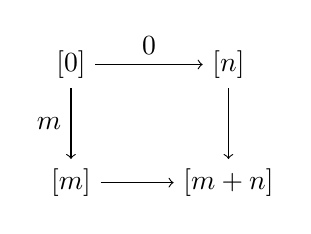
\begin{tikzpicture}[baseline = 0.75cm]
	\node (LT) at (0, 1.5) {$[0]$};
	\node (LB) at (0, 0) {$[m]$};
	\node (RT) at (2, 1.5) {$[n]$};
	\node (RB) at (2, 0) {$[m+n]$};
	\draw [->] (LT) -- node [left] {$m$} (LB);
	\draw [->] (LT) -- node [above] {$0$} (RT);
	\draw [->] (RT) -- node [right] {$$} (RB);
	\draw [->] (LB) -- node [below] {$$} (RB);
	%\node at (0.5, 1) {$\ulcorner$};
	%\node at (1.5, 0.5) {$\lrcorner$};
\end{tikzpicture}
\end{equation}
where $0: [0] \to [n]$ and $m: [0] \to [m]$ denote the first and last vertices, respectively. 

Let $\Gamma$ be the category introduced by Segal in \cite{Segal-Categories and Cohomology Theories}. The objects of $\Gamma$ are finite (unpointed, possibly empty) sets, and a morphism in $\Gamma$ from $A$ to $B$ consists of a function $f: A \to P(B)$, satisfying $f(x) \cap f(y) = \emptyset$ if $x \neq y$, where $P(B)$ denotes the power-set of $B$. The opposite category $\Gamma^\textrm{op} \simeq Fin_*$ is the category of finite pointed sets. There is a functor $\varphi:\Delta \to \Gamma$, which sends $[m]$ to the set $(m) = \{ 1, 2, \dots, m\}$, and sends $f: [m] \to [n]$ to the function $\varphi_f: i \in (m) \mapsto \{ j \in (n) \; | \: f(i-1) < j \leq f(i) \}$. For each element $a \in A$, there exists a canonical map $i_a: (1) \to A$, which is defined by setting $i_a(1) = \{a\} \subseteq A$. 


Let $C$ be a category. The category of {\em simplcial objects of $C$} is the functor category $Fun(\Delta^\textrm{op}, C)$. A {\em category internal to $C$} is such a simplicial object $X$, such that the diagrams induced by those in equation (\ref{Eqn:Segal-Co-Map}),
\begin{center}
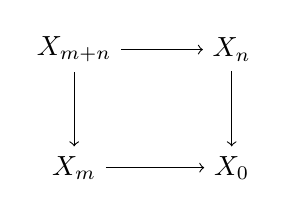
\begin{tikzpicture}
	\node (LT) at (0, 1.5) {$X_{m+n}$};
	\node (LB) at (0, 0) {$X_m$};
	\node (RT) at (2, 1.5) {$X_n$};
	\node (RB) at (2, 0) {$X_0$};
	\draw [->] (LT) -- node [left] {$$} (LB);
	\draw [->] (LT) -- node [above] {$$} (RT);
	\draw [->] (RT) -- node [right] {$$} (RB);
	\draw [->] (LB) -- node [below] {$$} (RB);
	%\node at (0.5, 1) {$\ulcorner$};
	%\node at (1.5, 0.5) {$\lrcorner$};
\end{tikzpicture}
\end{center}
are a pull-back diagrams. For a general simplicial object, these commuting squares will be called {\em Segal squares}. Hence a category internal to $C$ is a simplicial object in which every Segal square is a pull-back square. 

This may be contrasted with the notion of a category internal to $C$, which consists of a {\em set} of objects together with hom objects $Hom(x,y) \in C$ (as opposed to an object $X_0 \in C$ of objects). Under certain conditions these notions may be related. Recall that a category is {\em extensive} (or {\em infinitary extensive}) if it admits small coproducts and coproducts are disjoint and stable under pullback. If $C$ is an extensive category with a terminal object, then a category enriched in $C$ is merely an internal category $X$ in which the object $X_0$ is {\em discrete}, i.e. a coproduct of terminal objects. Examples of extensive categories with terminal objects include the categories of sets, spaces, small categories,\CSP{Is the category of small categories really extensive?} any category of presheaves, and more generally any Grothendieck topos. 

\begin{example}
	A {\em strict 2-category} is a category enriched in categories.
\end{example}

\begin{definition}
	Let $sSet$ denote the category of simplicial sets. An {\em $n$-fold simplicial space} is a functor $X: (\Delta^\textrm{op})^{\times n} \to sSet$. A {\em $\Gamma$-$n$-fold simplicial space} is a functor $X: \Gamma^\textrm{op} \times (\Delta^\textrm{op})^{\times n} \to sSet$.
\end{definition}

The categories of $n$-fold simplicial spaces and $\Gamma$-$n$-fold simplicial spaces admit combinatorial model structures which give robust theories of $(\infty, n)$-categories and symmetric monoidal $(\infty, n)$-categories, respectively. This is the context in which the cobordism hypothesis has been proven and is the context in which we frame our results. The fibrant objects of these model categories are the so-called $n$-fold complete Segal spaces and special $\Gamma$-$n$-fold complete Segal spaces, respectively. These fibrant objects enjoy many desirable properties. For example, the weak equivalences between fibrant objects are precisely the levelwise weak equivalences. Also many related constructions, like the homotopy category of an $(\infty, n)$-category, have simple direct descriptions for these fibrant objects. 

On the other hand, many examples occurring {\em in nature} do not arise as $n$-fold complete Segal spaces or special $\Gamma$-$n$-fold complete Segal spaces. For example in \cite{Lurie}, the $(\infty, n)$-category of cobordisms is constructed as a $n$-fold Segal space which is {\em not} complete. There are a number classes of $n$-fold simplicial spaces which are intermediary between general $n$-fold simplicial spaces and the fibrant $n$-fold complete Segal spaces. For many purposes these intermediary objects are just as good as their fibrant replacement. One such intermediate notion is that of $n$-fold Segal category, and it is this intermediate notion to which we now turn. 
%\begin{definition}
%	An $n$-fold simplicial space $X$ is {\em essentially constant} if, when regarded as a functor $X: (\Delta^\textrm{op})^{\times n} \to h\textrm{-}(sSet)$, it is equivalent to a constant functor, where $h\textrm{-}(sSet)$ denotes the homotopy category of simplicial sets.  
%\end{definition}
%
We may regard any $n$-fold simplicial space as a simplicial object in $(n-1)$-fold simplicial spaces. A $0$-fold simplicial space is understood to be a simplicial set. 

\begin{definition}
	A $0$-fold simplicial space (i.e. a simplicial set) is a {\em $0$-fold Segal category} if it is a Kan complex. An $n$-fold simplicial space $X$, regarded as a simplicial object $X_\bullet$ in $(n-1)$-fold simplicial spaces is an {\em $n$-fold Segal category} if the following conditions are satisfied
		\begin{enumerate}
			\item The $(n-1)$-fold simplicial space $X_0$ is constant and discrete.
			\item Each of the $(n-1)$-fold simplicial spaces $X_k$ is an $(n-1)$-fold Segal category.
			\item For every $m, k$, the Segal square,
			\begin{center}
			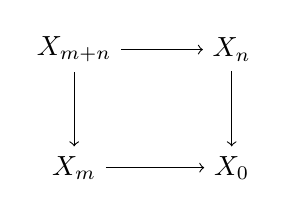
\begin{tikzpicture}
				\node (LT) at (0, 1.5) {$X_{m+n}$};
				\node (LB) at (0, 0) {$X_m$};
				\node (RT) at (2, 1.5) {$X_n$};
				\node (RB) at (2, 0) {$X_0$};
				\draw [->] (LT) -- node [left] {$$} (LB);
				\draw [->] (LT) -- node [above] {$$} (RT);
				\draw [->] (RT) -- node [right] {$$} (RB);
				\draw [->] (LB) -- node [below] {$$} (RB);
				%\node at (0.5, 1) {$\ulcorner$};
				%\node at (1.5, 0.5) {$\lrcorner$};
			\end{tikzpicture}
			\end{center}
			is a homotopy pull-back square of $(n-1)$-fold simplical spaces, computed with the $(\infty, n-1)$-model structure.
		\end{enumerate}
	\end{definition}
This final condition requires some explanation. The Segal square must realize $X_{m+n}$ as the homotopy fiber product $X_m \times_{X_0}^h X_n$, and this homotopy fiber product must be computed in the $(\infty, n-1)$-category model structure on $(n-1)$-fold simplicial sets. Moreover $X_{m+n}$ may not be levelwise equivalent to this homotopy fiber product, but merely weakly equivalent in this model structure. Fortunately, we require that $X_0$ is a discrete $(n-1)$-fold simplcial space. In this case the homotopy fiber product simplifies and is merely the ordinary fiber product. Thus condition (3) is equivalent to:

\begin{enumerate}
	\item [(3')] For every $m$ and $k$ the Segal map $X_{m+n} \to X_m \times_{X_0} X_n$ is an equivalence of $(n-1)$-fold Segal categories. 
\end{enumerate}

Moreover equivalences between $n$-fold Segal categories admit a fairly tractable inductive recognition principle. To describe this me must introduce a few auxiliary concepts. Let $X$ be an $n$-fold Segal category. Recall that $X_0$ is a constant discrete simplicial space, and so may be regarded as a set. We call the elements of $X_0$ objects of $X$. 
Inductively we will define three functorial constructions:
\begin{itemize}
	\item For every pair of objects $a,b \in X_0$, an $(n-1)$-fold Segal category $Hom_X(a,b)$.
	\item A category $\mathit{h}X$, called the {\em homotopy category} of $X$.
	\item A set $\pi_0 X$, which is the set of isomorphism classes of objects of $\mathit{h}X$. 
\end{itemize}
Once we have these constructions, equivalences of $n$-fold Segal categories are easy to recognize: they are precisely those maps $f:X \to Y$ of $n$-fold simplicial spaces which induce equivalences of homotopy categories $\mathit{h}f:\mathit{h}X \to \mathit{h}Y$ and which induce equivalences of hom $(n-1)$-fold Segal categories $Hom_X(a,b) \to Hom_Y(fa, fb)$ for every pair of objects $a,b \in X_0$. 

Given a pair objects $a,b \in X_0$ in an $n$-fold Segal category $X$, the hom $(n-1)$-fold Segal category $Hom_X(a,b)$ is defined to be the fiber over $(a,b) \in X_0 \times X_0$ of the map $(d_0, d_1): X_1 \to X_0 \times X_0$.  
\begin{center}
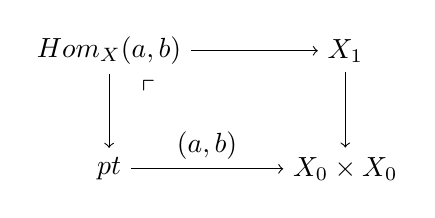
\begin{tikzpicture}
	\node (LT) at (0, 1.5) {$Hom_X(a,b)$};
	\node (LB) at (0, 0) {$pt$};
	\node (RT) at (3, 1.5) {$X_1$};
	\node (RB) at (3, 0) {$X_0\times X_0$};
	\draw [->] (LT) -- node [left] {$$} (LB);
	\draw [->] (LT) -- node [above] {$$} (RT);
	\draw [->] (RT) -- node [right] {$$} (RB);
	\draw [->] (LB) -- node [above] {$(a,b)$} (RB);
	\node at (0.5, 1) {$\ulcorner$};
	%\node at (1.5, 0.5) {$\lrcorner$};
\end{tikzpicture}
\end{center}
The homotopy category $\mathit{h}X$ has the same object set $X_0$, and the morphisms set between two objects is given as the set $Hom_{\mathit{h}X}(a,b) := \pi_0 Hom_X(a,b)$. For every triple of objects $a,b,c \in X_0$ we have a similar $(n-1)$-fold Segal category $Hom_X(a,b,c)$ which is defined as the fiber in $X_2$ over the point $(a,b,c)$ in $X_0 \times X_0 \times X_0$. Since $X$ is an $n$-fold Segal category we have induced maps of $(n-1)$-fold Segal categories,
\begin{equation*}
	Hom_X(a,b) \times Hom_X(b,c) \stackrel{\simeq}{\longleftarrow} Hom_X(a,b,c) \stackrel{}{\longrightarrow} Hom_X(a,c).
\end{equation*}
Composition in $\mathit{h}X$ is given by the induced map of sets,
\begin{equation*}
	 Hom_{\mathit{h}X}(a,b) \times Hom_{\mathit{h}X}(b,c) \cong \pi_0 Hom_X(a,b,c)\to \pi_0 Hom_X(a,c) = Hom_{\mathit{h}X}(a,c).
\end{equation*}




%If the $n$-fold Segal spaces $X_k$ are fibrant, that is complete, then these problems disappear. Weak equivalences between fibrant objects are computed levelwise, as are homotopy fiber products. 

%Thus in general we are left with the embarrassing responsibility of computing the correct homotopy fiber product $X_m \times_{X_0}^h X_n$, and showing that the canonical map from $X_{m+n}$ is a weak equivalence of $(\infty, n-1)$-categories. Fortunately there is another subclass of $n$-fold Segal spaces for which these two operations are relatively easy to perform: The {\em $n$-fold Segal categories}.

\begin{definition}
%   A $0$-fold Segal category is a Kan complex. An {\em $n$-fold Segal category} is an $n$-fold Segal space which satisfies
%   \begin{enumerate}
%   	\item $X_0$ is discrete, and
%   	\item for each $n$, $X_n$ is an $(n-1)$-fold Segal category. 
%   \end{enumerate}
	A {\em special $\Gamma$-$n$-fold Segal category} is a $\Gamma$-$n$-fold simplicial space $X$, which we view as a functor from $\Gamma^\textrm{op}$ to $n$-fold simplcial spaces, such that the following conditions are satisfied. 
	\begin{enumerate}
		\item $X_A$ is an $n$-fold Segal category for each $A \in \Gamma$. 
		\item For each set $A \in \Gamma$ (possibly empty) the canonical map,
		\begin{equation*}
			\prod_{a \in A} i_a^*: X_A \to \prod_{a \in A} X_{(1)}
		\end{equation*}
		is an equivalence of $n$-fold Segal categories. %\CSP{Should we also add the $X_{(0)} = pt$? We get $X_{(0)} \simeq pt$ for free.}
	%	\item (optional) The previous axiom implies that $X_\emptyset \simeq pt$. We assert that $X_\emptyset = pt$. 
	\end{enumerate}
\end{definition}

%The first significant advantage of $n$-fold Segal categories follows from the fact that the homotopy fiber product over a discrete base, for example $X_m \times_{X_0}^h X_n$ when $X$ is an $n$-fold Segal category, agrees with the ordinary fiber product. Thus we many avoid a lengthly discussion of the model structure of $n$-fold complete Segal spaces and work directly with ordinary fiber products.

%We must also identify the weak equivalences between $n$-fold Segal categories. These admit a fairly direct inductive description in terms of the homotopy category $hX$ of an $n$-fold Segal category.



%-----


%The {\em homotopy pull-back} of $n$-fold simplicial spaces may be inductively defined as follows. For $0$-fold simplicial spaces a homotopy pull-back is a homotopy pull-back in the standard model structure on simplicial sets. For general $n$-fold simplicial spaces $W$, $X$, $Y$, and $Z$, a diagram 
%\begin{center}
%\begin{tikzpicture}
%	\node (LT) at (0, 1.5) {$W$};
%	\node (LB) at (0, 0) {$X$};
%	\node (RT) at (2, 1.5) {$Y$};
%	\node (RB) at (2, 0) {$Z$};
%	\draw [->] (LT) -- node [left] {$$} (LB);
%	\draw [->] (LT) -- node [above] {$$} (RT);
%	\draw [->] (RT) -- node [right] {$$} (RB);
%	\draw [->] (LB) -- node [below] {$$} (RB);
%	%\node at (0.5, 1) {$\ulcorner$};
%	%\node at (1.5, 0.5) {$\lrcorner$};
%\end{tikzpicture}
%\end{center}
%is a homotopy pull-back diagram if and only if for each $n$ the diagram 
%\begin{center}
%\begin{tikzpicture}
%	\node (LT) at (0, 1.5) {$W_n$};
%	\node (LB) at (0, 0) {$X_n$};
%	\node (RT) at (2, 1.5) {$Y_n$};
%	\node (RB) at (2, 0) {$Z_n$};
%	\draw [->] (LT) -- node [left] {$$} (LB);
%	\draw [->] (LT) -- node [above] {$$} (RT);
%	\draw [->] (RT) -- node [right] {$$} (RB);
%	\draw [->] (LB) -- node [below] {$$} (RB);
%	%\node at (0.5, 1) {$\ulcorner$};
%	%\node at (1.5, 0.5) {$\lrcorner$};
%\end{tikzpicture}
%\end{center}
%is a homotopy pull-back diagram of $(n-1)$-fold simplicial spaces. Thus homotopy fiber products are computed `levelwise'. In particular if $Z$ is a discrete $n$-fold simplicial space, then the homotopy fiber product is levelwise homotopy equivalent to the usual fiber product. 



 


	
	
%	We now inductively define a class of objects called {\em $n$-fold Segal spaces} as well as a collection of maps of $n$-fold Segal spaces called {\em weak equivalences}. For $0$-fold simplicial spaces Segal spaces are the Kan complexes. The weak equivalences between $0$-fold simplicial spaces are the weak equivalences of simplicial sets.  
	

%\CSPcomm{[There is a model category of $\Gamma$-$n$-fold complete Segal spaces which models symmetric monoidal $(\infty, n)$-categories]. The is a completion functor (fibrant replacement), so it is enough to produce a $\Gamma$-$n$-fold simplicial space. We produce a Segal one.}

\subsubsection*{The $\Gamma$-$3$-fold Segal Category of Tensor Categories}

Our construction of the $\Gamma$-$3$-fold Segal Category of Tensor Categories will proceed in several stages. We will first describe how a strict 2-category gives rise to a 2-fold Segal category. This can be regarded as a 2-categorical nerve. Then we will construct explicitly $TC$ as a simplicial object in the category of strict 2-categories. Applying the previous 2-categorical nerve yields a 3-fold simplcial space which is shown to be a 3-fold Segal category. A variation on these constructions yields the $\Gamma$-3-fold Segal space $TC$. 

%\begin{definition}
%	A strict 2-category is a category object $(C_1 \rightrightarrows C_0)$ in categories such that the category of objects $C_0$ is discrete (i.e. its only morphisms are identities). 
%\end{definition}


A strict 2-category gives rise to a simplicial category $C_\bullet$ whose $n^\textrm{th}$ category is given by the usual formula
\begin{equation*}
	C_n := \sqcup_{x_0, x_1, \dots, x_n \in C_0} \hom_C(x_0, x_1) \times \hom_C(x_1, x_2) \times \cdots \times \hom_C(x_{n-1}, x_n).
\end{equation*}
We obtain a 2-fold simplicial set by applying the standard nerve construction to each of these categories. Finally, we obtain a 2-fold simplcial space $NC_{\bullet \bullet}$ by viewing a set as a discrete simplicial space. The nerve of a 1-category, viewed as a simplicial space, automatically satisfies the conditions to be a Segal category. Moreover $NC_{\bullet \bullet}$ is a 2-fold Segal category. 
\footnote{Alternatively, one may start with the simplicial category $C_\bullet$, as before and apply the {\em complete Segal space nerve} to each of the categories $C_n$. The $k^\text{th}$ space of this simplicial space $N^{CSS}_\bullet C_n$ is obtained by first constructing the functor category $Fun([k], C_n)$, then throwing away the non-invertible natural transformations, and finally applying the classifying space functor to the resulting groupoid. This alternative has the advantage that it produces a {\em complete} Segal space $N^{CSS} C_n$. However for our purposes these are equivalent constructions as the canonical map $N C_n \to N^{CSS} C_n$ is a weak equivalence in the complete Segal space model structure. 
%[Cite the Joyal Teinery paper for the Quillen equivalence between Segal spaces and Quasi-categories]
}

The 3-fold Segal Category of tensor categories is first constructed as a simplicial object $TC$ in the 1-category of strict 2-categories (and strict 2-functors). The 3-fold Segal category is then obtained by applying the above 2-categorical nerve levelwise. For each $[n] \in \Delta$ we have a strict 2-category $TC_n$ defined as follows. The objects, 1-morphism, and 2-morphisms of $TC_n$ correspond to certain labelings of the $n$-simplex $[n]$. The objects of $TC_n$ consist of:
\begin{itemize}
	\item For each vertex $i$ of $[n]$, a tensor category $A_i$. 
	\item For each edge $ij$ of $[n]$, an $A_i$-$A_j$-bimodule category $M_{ij}$.
	\item For each 2-simplex $ijk$ of $[n]$, an $A_j$-balanced functor of $A_i$-$A_k$-bimodule categories 
	\begin{equation*}
		\varphi_{ijk}: M_{ij} \times M_{jk} \to M_{ijk},
	\end{equation*}
	 which realizes $M_{ik}$ as the tensor product $M_{ik} \simeq M_{ij} \otimes_{A_j} M_{jk}$. 
	\item For each 3-simplex $ijk\ell$ of $[n]$, a natural transformation of $A_j$/$A_k$-balanced $A_i$-$A_\ell$-bimodule functors 
	\begin{equation*}
		\alpha_{ijk \ell}: \varphi_{i k \ell} \circ (\varphi_{ijk} \times id_{M_{k\ell}}) \to \varphi_{ij \ell} \circ (id_{M_{ij}} \times \varphi_{jk\ell}).
	\end{equation*}
	 %inducing the identity natural isomorphism of the canonical equivalence $(M_{ij} \otimes_{A_j} M_{jk}) \otimes_{A_k} M_{k\ell} \simeq M_{ij} \otimes_{A_j}( M_{jk} \otimes_{A_k} M_{k\ell}).$
	\item such that for each $4$-simplex $ijk\ell m$ of $[n]$, the following pentagon identity is satisfied:
	\begin{align*}
		\text{(to be added)}  \\ [\varphi_{ijm} * (id_{M_{ij}} \times \alpha_{jk\ell m})] \circ [\alpha_{ij\ell m} * (id_{M_{ij}} \times \varphi_{jk\ell} \times id_{M_{\ell m}})] \circ [\varphi_{i \ell m} * ( \alpha_{ijk \ell} \times id_{M_{\ell m}})] = ...
	\end{align*} \CSPcomm{Need to finish the pentagon equation.}
\end{itemize}
Let $X$ and $Y$ be two objects in $TC_n$. The 1-morphisms of $TC_n$ from $X$ to $Y$ consist of labeled $n$-simplices where:
\begin{itemize}
	\item For each vertex $i$ of $[n]$, the tensor category $A_i^X$ and $A^Y_i$ agree identically. 
	\item For each edge $ij$ of $[n]$, an $A_i$-$A_j$-bimodule functor 
	\begin{equation*}
		F_{ij}: M_{ij}^X \to M_{ij}^Y.
	\end{equation*}
	\item For each 2-simplex $ijk$ of $[n]$, a natural isomorphism of $A_j$-balanced $A_i$-$A_k$-bimodule functors
	\begin{equation*}
		\xi_{ijk}: \varphi_{ijk}^Y \circ (F_{ij} \times F_{jk}) \to F_{ik} \circ \varphi_{ijk}^X
	\end{equation*}
	\item Such that for each 3-simplex $ijk\ell$ of $[n]$, the equation
	\begin{equation*}
			\text{(to be added)}
	\end{equation*}
	is satisfied.
\end{itemize} 
Let $F,G: X \to Y$ be two parallel 1-morphisms in $TC_n$. The 2-morphisms from $F$ to $G$ in $TC_n$ consist of:
\begin{itemize}
	\item For each edge $ij$ of $[n]$, a natural transformation of $A_i$-$A_j$-bimodule functors
	\begin{equation*}
		\theta_{ij}: F_{ij} \to G_{ij}.
	\end{equation*}
	\item Such that for each 2-simplex $ijk$ of $[n]$, the equation
	\begin{equation*}
		\xi_{ijk}^G \circ (  id_{\varphi_{ijk}^Y} * \theta_{ij} \times \theta_{jk}) = (\theta_{ik} * id_{\varphi_{ijk}^X} ) \xi_{ijk}^F
	\end{equation*}
	is satisfied. 
\end{itemize}


(face and degeneracy maps. (forgetting and repeating))

Let $A$ be a finite set. Let $P(A)$ denote the power set of $A$, viewed as a poset via inclusion. Define $TC(n,A)$ to be the full sub-2-category of the strict functor 2-category $Fun(P(A), TC_n)$ consisting of those functors, natural transformations, and modifications which satisfy the following conditions. If $S_0$ and $S_1$ are disjoint subsets of $A$, then the induced map 
\begin{equation*}
	X(S_0) \times X(S_1) \to X(S_0 \sqcup S_1) \quad \text{ (need to finish)}
\end{equation*} 
\CSPcomm{Wait, don't the morphism in $TC_n$ fix the vertex tensor categories by definition? So then an inclusion doesn't correspond to a map in $TC_n$?}

If $f:A \to P(B)$ is a morphism in $\Gamma$, then we get a functor $f^*: TC(n, B) \to TC(n,A)$ which on objects sends $X \in TC(n,B)$ to the assignment $f^*X(S) = X( \cup_{s \in S} f(s))$. Since $f$ sends disjoint unions to disjoint unions, this formula does indeed define an object of $TC(n,A)$. 

\CSPcomm{Maybe I should reverse the order of these discussions. First discuss $P(A)$ and construct "bilinear sequences" which would consist of sequences of objects linear categories index by the subsets of $A$, and satisfying the "Deligne condition" for disjoint unions. (is this the right term? Maybe Segal condition?). Then show this has its own Deligne tensor product (essentially objectwise). So then we get the notion of tensor object and also module and bimodule objects which consist of sequences of tensor categories or bimodule categories. Finally We can just export the above definition be replacing $X$ and its ilk by objects in the $A$ sequences. Lastly, we just need to observe that this gives a  Gamma simplicial 2-category.}

%--------- \CSPcomm{I need to edit the below.}
%
%\begin{itemize}
%	\item The $0^\text{th}$ 2-category is the discrete collection tensor categories viewed as a discrete 2-category. 
%	\item The $1^\text{st}$ 2-category consists of the disjoint union over all pairs of tensor categories $A$ and $B$ of the 2-categories of $A$-$B$-bimodule categories, functors, and natural transformations. 
%	\item The $2^\text{nd}$ 2-category consists of a disjoint union over all triples of tensor categories $A$, $B$, $C$ of certain 2-categories $TC_2(A,B,C)$. These 2-categories consists of triples of bimodules $ \bimod{A}{L}{B}$, $ \bimod{B}{M}{C}$, $ \bimod{A}{N}{C}$, together with a $B$-balanced $A$-$C$-linear functor $L \times M \to N$ inducing an equivalence $\bimod{A}{L \boxtimes_B M }{C} \cong  \bimod{A}{N }{C}$. The 1-morphisms and 2-morphisms are the obvious ones. 
%	\item The $3^\text{rd}$ 2-category consists of the disjoint union ...
%	\item 
%	\item The higher 2-categories are completely determined by their restriction to ... 
%\end{itemize}




---------

\CDcomm{Formalism for 3-categories.}

\CDcomm{Formalism for symmetric monoidal 3-categories.}
A symmetric monoidal category is the same as a functor $Fin_* \to \Cat$ which sends coproducts to products. A symmetric monoidal 3-category is a functor $Fin_* \to 3\text{-}\Cat$ which sends coproducts to products.

\CDcomm{Definition of TC.}
\CDcomm{[Objects of TC are \emph{idempotent complete linear categories}.  Morphisms are ..., 2-morphism are ..., 3-morphism are ...]}


\begin{remark}
It is worth keeping in mind, and separating, the two key conceptual differences between the setting of tensor categories and the setting of ordinary algebra.  The first difference is, obviously, that we have categorified---the underlying objects are now longer sets but categories.  The second difference is that the elements of the objects no longer have additive inverses---that is objects of a tensor category, unlike elements of an algebra, needn't be additively invertible.  For many purposes and arguments, the second is the more serious and problematic difference.
\end{remark}

\subsection{Multi-Fusion categories} \label{sec-tc-fusion}

\CD{CD continues to vote for using 'fusion' rather than 'multifusion'}

\begin{definition}
A \emph{fusion category} is a tensor category $\cC$ satisfying the following conditions:
\begin{enumerate}
\item For all objects $a, b \in \cC$, the vector space $\Hom(a,b)$ is finite dimensional.
\item The category $\cC$ is semisimple, with finitely many simple objects.
\item For every object $a \in \cC$, there exists an object $\ld{a} \in \cC$ that is a left dual for $a$ and there exists an object $\rd{a} \in \cC$ that is a right dual for $a$.
\end{enumerate}
\end{definition}

\begin{remark}
Here for brevity we use ``fusion category" to refer to what has elsewhere gone under the name ``multi-fusion category".
\end{remark}

\begin{proposition}
If $\cC$ is a fusion category, then there exist monoidal functors $\ld{(-)} : \cC \ra \cC^{\mop}$ and $\rd{(-)} : \cC \ra \cC^{\mop}$ whose values on any object $a \in \cC$ are respectively a left dual object $\ld{(a)}$ and a right dual object $\rd{(a)}$ for $a$.
\end{proposition}

\begin{proof}
Define the functor $\ld{(-)}$ on objects by picking for each object $a \in \cC$ a left dual object $\ld{a} \in \cC$.  Also pick a unit map $u: \ld{a} \; a \ra 1$ and a counit map $v: 1 \ra a \; \ld{a}$ giving $\ld{a}$ the structure of a left dual to $a$.  Define the functor $\ld{(-)}$ on a morphism $f: a \ra b$ by $\ld{(f)} := (u_b \cdot \id_{\ld{a}}) (\id_{\ld{b}} \cdot f \cdot \id_{\ld{a}}) (\id_{\ld{b}} \cdot v_a)$.  (This morphism $\ld{(f)}$ is called the \emph{mate} of $F$.)  Next we want to see that this functor is monoidal.  Observe that the morphisms $\ld{b} \; \ld{a} \; a \; b \xra{u_a} \ld{b} \; b \xra{u_b} 1$ and $1 \xra{v_a} a \; \ld{a} \xra{v_b} a \; b \; \ld{b} \; \ld{a}$ show that $(\ld{b} \; \ld{a})$ is a left dual to $(a b)$.  There is therefore a uniquely determined isomorphism from $(\ld{b} \; \ld{a})$ to $\ld{(a b)}$.  These isomorphisms provide the left dual functor with a monoidal structure.  The right dual functor is analogous.  % In principle, need to check naturality and hexagon for those isos.
\end{proof}
% This fact is asserted in Bruce's thesis; the functor part is mentioned in Selinger Eg 4.4.

\begin{remark}
The monoidal functor $\ld{(-)}: \cC \ra \cC^{\mop}$ is an equivalence of tensor categories; the inverse functor is $\rd{(-)}: \cC^{\mop} \ra \cC$.
\end{remark}

\begin{definition}
A fusion category $\cC$ is \emph{pivotal} if the double left dual functor $\ldd{(-)}: \cC \xra{\ld{(-)}} \cC^{\mop} \xra{\ld{(-)}} \cC$ is equivalent to the identity functor as a monoidal functor.
\end{definition}

In other words, a fusion category is pivotal if the left dual functor $\ld{(-)}: \cC \ra \cC^{\mop}$ and the right dual functor $\rd{(-)}: \cC \ra \cC^{\mop}$ are monoidally equivalent.


\section{Local Field Theory in Dimension Three} \label{sec-lft}

\subsection{Dualizability in 3-categories} \label{sec-lft-dual}
.
\CD{I guess the content of this section should be dictated by what we need for sections 4,5,6.  What is that?}

[Adjunction convention: $\bimod{C}{M}{D} \adj  \bimod{D}{N}{C}$ if there are $M \dtimes_D N \ra C$ and $D \ra N \dtimes_C M$ satisfying the S relations.] 

\CSPcomm{Set up terminology for evaluation and coevaluation.}


%\CSP{This proposition is stated as a remark, without proof in Jacob's paper.}

\begin{proposition}[Lurie, Remark 3.4.22] \label{prop-ambiadjoints}
	Let $\cA$ be a symmetric monoidal 3-category. Let $f: x \to y$ be a 1-morphism in $\cA$, and suppose that $f$ admits a right adjoint $f^R$,  so we have unit and counit maps $u:id_x \to f^R \circ f$ and $v:f \circ f^R \to id_y$. If $u$ and $v$ admit left adjoints $u^L$ and $v^L$, then $u^L$ and $v^L$ exhibit $f^R$ also as a left adjoint to $f$. 
\end{proposition}

\begin{proof}
\CDcomm{[Should we include a proof?]} \CSPcomm{Of Course we should include a proof. Jacob omits one, so there is none in the literature, plus we need it as a substitute for the cob hypothesis for our applications to finite tensor cats.}

By assumption we are given 3-morphisms,
\begin{align*}
	\varepsilon_v: v^L \circ v & \Rightarrow id_{f \circ f^R} \\
	\eta_v: id_{id_y} & \Rightarrow v \circ v^L \\
	\varepsilon_u: u^L \circ u & \Rightarrow id_{id_x} \\
	\eta_u: id_{f^R \circ f} & \Rightarrow  u \circ u^L
\end{align*}
which satisfy the Zig-Zag identities:
\begin{align*}
	 id_v  &= (id_v * \varepsilon_v) \circ (\eta_v * id_v)  \\
	 id_{v^L}  &= (\varepsilon_v * id_{v^L} ) \circ (id_{v^L} * \eta_v)  \\
	 id_u  &= (id_u * \varepsilon_u) \circ (\eta_u * id_u)  \\
	 id_{u^L}  &= (\varepsilon_u * id_{u^L} ) \circ (id_{u^L} * \eta_u).  
\end{align*}
We must show that the following Zig-Zag identities hold:
\begin{align*}
	 (id_{f} * u^L) \circ (v^L * id_{f} ) & \cong id_{f} \\
 	 (u^L * id_{f^R}) \circ (id_{f^R} * v^L) & \cong id_{f^R} 
\end{align*}
By assumption we may also choose isomorphisms as follows:
\begin{align*}
	\alpha: id_f &\stackrel{\cong}{\to} (v * id_f) \circ (id_f * u) \\
	\beta: id_{f^R} &\stackrel{\cong}{\to} (id_{f^R} * v) \circ (u * id_{f^R} ).
\end{align*}
Then the required isomorphisms are given by the following composites:
\begin{align*}
	(id_{f} * u^L) \circ (v^L * id_{f} )
		& \cong id_f \circ (id_{f} * u^L) \circ (v^L * id_{f} ) \\
		& \stackrel{\alpha}{\cong} (v * id_f) \circ (id_f * u) \circ (id_{f} * u^L) \circ (v^L * id_{f} ) \\
		&  \stackrel{\varepsilon_u }{\Rightarrow} (v * id_f) \circ (v^L * id_{f} ) \\
		& \stackrel{\varepsilon_v }{\Rightarrow} id_{f},  \\
	(u^L * id_{f^R}) \circ (id_{f^R} * v^L) 
		& \cong  id_{f^R} \circ (u^L * id_{f^R}) \circ (id_{f^R} * v^L)  \\
		& \stackrel{\beta}{\cong}  (id_{f^R} * v) \circ (u * id_{f^R} )  \circ (u^L * id_{f^R}) \circ (id_{f^R} * v^L) \\
		& \stackrel{\varepsilon_u }{\Rightarrow} (id_{f^R} * v) \circ (id_{f^R} * v^L) \\
		& \stackrel{\varepsilon_v }{\Rightarrow} id_{f^R}.
\end{align*}
\end{proof}

In particular, if you are in a situation where you happen to know a priori that the 2-morphisms $u$ and $v$ will have left adjoints, then you know that any adjoint to the 1-morphism $f$ will be ambidextrous.  % This proposition gets used in the Remark in the section computing the Serre automorphism.

\subsection{Structure groups of 3-manifolds} \label{sec-lft-struc}

\begin{definition}
An \emph{unstable structure} for $n$-dimensional vector bundles is a space $T$ together with a fibration $f: T \ra BO(n)$.  A $T$-structure on an n-dimensional vector bundle $V$ on $X$ is a lift of the classifying map $X \xra{V} BO(n)$ along $f$ to $T$.

A \emph{stable structure} is a space $S$ together with a fibration $f: S \ra BO$.  An $S$-structure on an n-dimensional vector bundle $V$ on $X$ is a lift of the composite map $X \xra{V} BO(n) \ra BO$ along $f$ to $S$.
\end{definition}
\CD{Are you happy with this def? Ie without mentioning the group structure on $G \ra O$?}

The discussion in this section records material that was utilized implicitly in the obstruction theory analysis of the first author with Bartels and Henriques~\cite{bdh}.
\CD{This sentence isn't an attempt to claim credit, but to give Andre the credit he deserves for helping sort this stuff out.  There might be a better way or spot to do it.}

%\subsubsection{Unstable structures}

We describe six unstable structures for 3-dimensional vector bundles, namely \emph{orientation}, \emph{spin structure}, \emph{orpo structure}, \emph{2-framing}, \emph{string structure}, and \emph{framing}.

\begin{definition}
The following six spaces, together with the obvious maps to $BO(3)$, define the aforementioned unstable bundle structures:
\begin{itemize}
\item[Or:] $BSO(3)$
\item[Spin:] $BSpin(3) := \hofib(BSO(3) \xra{w_2} K(\ZZ/2,2))$
\item[Orpo:] $BOrpo(3) := \hofib(BSO(3) \ra BSO \xra{p_1} K(\ZZ,4))$
\item[2-Frame:] $B\Omega(Spin(6)/SO(3))$
\item[String:] $BString(3) := \hofib(BSpin(3) \ra BSpin \xra{(p_1)/2} K(\ZZ,4))$
\item[Frame:] $*$
\end{itemize}
\end{definition}

\nid In the definition of 2-Frame, the inclusion from $SO(3)$ to $Spin(6)$ is the canonical lift of the map $SO(3) \ra SO(6)$ sending $\phi$ to $\phi \oplus \phi$; hence the idea of framing twice the vector bundle, hence the name.

\begin{remark}
``Orpo structure" is short for ``oriented $p_1$ structure", and sometimes goes under the name ``$p_1$ structure" in the literature.  Note that there is, however, a structure group where only $p_1$ has been killed, rather than $w_1$ and $p_1$, and that structure is itself sometimes refered to as a ``$p_1$ structure".  We won't have need for those $p_1$ structures and so do not discuss them; similarly we omit versions of $Pin$ structures.
\end{remark}

Orpo structures and 2-framings are different; for instance, the set of homotopy classes of parametrized families of the two structures on a vector bundle can be genuinely distinct.  However, as far individual tangential structures on a single 3-manifold are concerned, they are homotopically indistinguishable---this convergence no doubt has contributed to some of the confusion in the literature.
\begin{proposition}
There is a homotopy equivalence between the 4-coconnected covers of $BOrpo(3)$ and $B\Omega(Spin(6)/SO(3))$.  In particular, for a closed 3-manifold $M$, there is a bijection between the tangential orpo structures and the tangential 2-framings on $M$.
\end{proposition}
\CD{I mean the space where you killed $\pi_4$ and up --- that's ``4-coconnected"?}
\CDcomm{[Is there a canonical map from $B\Omega(Spin(6)/SO(3))$ to $BOrpo(3)$ or vice versa? Ie is the composite $B\Omega (Spin(6)/SO(3)) \ra BSO(3) \ra BSO \xra{p_1} K(\ZZ,4)$ trivial?  Is the composite $BOrpo(3) \ra BSO(3) \ra BSpin(6)$ trivial?  If so, adjust the above discussion to reflecct this.  If not, leave as is.]}
\CD{I haven't (re)checked the k-invariant between $\pi_2$ and $\pi_3$. We better do that.}
\CDcomm{[Ack, don't you need a 5-coconnected equivalence to get the bijection of tangential structures?  Or maybe you need a touch less than that.  Is it a 4- or 5-coconn equiv?  Maybe there is a more subtle reason why there is a bijection even if it isn't a 5-coconn equiv?]}

% Omit the proof.

Though the definition and analysis of these unstable structures on 3-dimensional vector bundles is elementary, there are potential pitfalls, so we record some information about them in rather pedantic detail.
\begin{proposition} \CD{Everything in this proposition should be carefully rechecked.}
.
\begin{enumerate}
%
\item
The homotopy groups $\pi_2$, $\pi_3$, $\pi_4$, and $\pi_5$ of the classifying spaces for the first five structure groups in question are as follows:
\begin{itemize}
\item[$BSO(3)$:] $\ZZ/2$, $0$, $\ZZ$, $\ZZ/2$
\item[$BSpin(3)$:] $0$, $0$, $\ZZ$, $\ZZ/2$
\item[$BOrpo(3)$:] $\ZZ/2$, $\ZZ/4$, $0$, $\ZZ/2$
\item[$Spin(6)/SO(3)$:] $\ZZ/2$, $\ZZ/4$, \CDcomm{$\ZZ/2$}, \CDcomm{?}
\item[$BString(3)$:] $0$, $0$, $0$, $\ZZ/2$
\end{itemize}
%
\item
The integral cohomology groups $H^3$, $H^4$, and $H^5$ of the stable and unstable orthogonal and spin classifying spaces are as follows:
\begin{itemize}
\item[$BSO(3)$:] $\ZZ/2$, $\ZZ$, $0$
\item[$BSpin(3)$:] $0$, $\ZZ$, $0$
\item[$BSO$:] $\ZZ/2$, $\ZZ$, $\ZZ/2$
\item[$BSpin$:] ...
\end{itemize}
%
\item 
On fourth integral cohomology, the maps among these classifying spaces are as follows:
\begin{itemize}
\item[$BSO(3) \ra BSO$:] \CDcomm{1}
\item[$BSpin(3) \ra BSO(3)$:] ...
\item[$BSpin \ra BSO$:] ...
\item[$BSpin(3) \ra BSpin$:] ...
\end{itemize}
As a result, the generator of $H^4(BSO(3);\ZZ)$ is $p_1/...$ and the generator of $H^4(BSpin(3);\ZZ)$ is $p_1/...$.
\end{enumerate}
\end{proposition}

\CDcomm{[In all this, the following weird fact (recheck) is relevant: $\pi_4(BSO(3) \xra{p_1} K(\ZZ,4)) = 4$, even though $p_1$ is a generator of $H^4(BSO(3);\ZZ)$.]}

\CDcomm{[This point of this proposition is to see what the generators of $H^4$ of $BSO(3)$ and $BSpin(3)$ are, since those determine the options for the unstable structure groups.]}

%\subsubsection{Stable structures}

Though in dimension 3 all the natural stable structures are equivalent, at least in unparametrized homotopy, to unstable structures, it is nevertheless worth mentioning them.  We describe the structures \emph{stable orientation}, \emph{stable spin structure}, \emph{stable orpo structure}, \emph{stable string structure}, and \emph{stably framed structure}.

\begin{definition}
The following five spaces, together with the obvious maps to $BO$, define the aforementioned stable bundle structures:
\begin{itemize}
\item[StOr:] $BSO$
\item[StSpin:] $BSpin$
\item[StOrpo:] $\hofib(BSO \xra{p_1} K(\ZZ,4))$
\item[StString:] $\hofib(BSpin \xra{(p_1)/2} K(\ZZ,4))$
\item[StFrame:] $*$
\end{itemize}
\end{definition}

\nid Note that for $X \in \{\Or, \Spin, \Orpo, \String\}$, a stable $X$ structure on a 3-dimensional vector bundle is exactly the same as an $X$ structure on a 3-dimensional vector bundle, because $BX(3)$ is by construction the homotopy pullback of $BO(3) \ra BO \la BX$.  This is not, however, the case for $X = \Frame$; indeed there is a substantial difference between a framing and a stable framing.  Nevertheless, as far as individual tangential structures on 3-manifolds are concerned, there is a homotopical coincidence between stably framed structures and stable string structures, therefore between stably framed structures and string structures.
\begin{proposition}
For $M$ a 3-manifold, the natural forgetful map from stably framed structures to stable string structures induces a bijection between the set of homotopy classes of stable framings on $M$ to the set of homotopy classes of stable string structures on $M$.
\end{proposition}



\section{Dualizability and fusion categories} \label{sec-dualfusion}


\subsection{Fusion categories are dualizable} \label{sec-df-fcd}


\subsubsection{Functors of finite semisimple module categories have adjoints} \label{sec-df-functors}

\CD{cf ENOPartII "Solution to item (1)"}

\begin{lemma}
Let $F: \bimod{\cC}{\cM}{\cD} \ra \bimod{\cC}{\cN}{\cD}$ be a functor of bimodule categories, and suppose the underlying functor $\tilde{F}: \cM \ra \cN$ of linear categories has an ambidextrous adjoint $\tilde{G}: \cN \ra \cM$.  Then $F$ has an ambidextrous adjoint $G: \bimod{\cC}{\cN}{\cD} \ra \bimod{\cC}{\cM}{\cD}$.
\end{lemma}

\begin{proof}
\CDcomm{Look at the wave}
\end{proof}

\begin{lemma}
Let $F: \bimod{\cC}{\cM}{\cD} \ra \bimod{\cC}{\cN}{\cD}$ be a functor of bimodule categories.  If $\cM$ and $\cN$ are semisimple categories with finitely many simple objects, then the functor $\tilde{F}: \cM \ra \cN$ of linear categories underlying $F$ has an ambidextrous adjoint.
\end{lemma}

\begin{proof}
\CDcomm{The ambidextrous adjoint $\rd{F}$ is given by the transpose of the entrywise dual of $F$.  That is, write $F$ as a matrix of vector spaces in terms of a chosen basis of simple objects for $M$ and $N$, then take the matrix of dual vector spaces, and take the transpose.}
...
\end{proof}

\begin{proposition} \label{prop-functadj}
A functor $F: \bimod{\cC}{\cM}{\cD} \ra \bimod{\cC}{\cN}{\cD}$ of bimodules categories has an ambidextrous adjoint if the linear categories $\cM$ and $\cN$ are semisimple with finitely many simple objects.
\end{proposition}

This proposition follows from the above two lemmas.


\subsubsection{Indecomposable modules with braided fusion commutant have adjoints} \label{sec-df-modules}


\begin{lemma} \label{lemma-invertible}
Let $\cC$ be a fusion category and $\cM$ an indecomposable $\cC$-module.  Let $\cC'$ denote the commutant of $\cC$ acting on $\cM$.  In this case the bimodule $\bimod{\cC}{\cM}{\cC'}$ is invertible, \CDcomm{with inverse $\bimod{\cC'}{\Hom_{\cC}(\cM,\cC)}{\cC}$}.
\end{lemma}

\begin{proof}
\CDcomm{See ENOPartIII Apr 7 "Lemma: When C is fusion" for a sketch.}

\CDcomm{Can this be shown only using that C is semisimple?}

\CDcomm{Crucial point: the inverse is given by $\Hom_C(M,C)$, right?.  Emphasize this.}
\end{proof}

In the situation of this lemma we will abbreviate the inverse \CDcomm{$\bimod{\cC'}{\Hom_{\cC}(\cM,\cC)}{\cC}$} of $\bimod{\cC}{\cM}{\cC'}$ by $\bimod{\cC'}{\cN}{\cC}$.

\begin{lemma} \label{lemma-conditional}
Let $\cC$ be a fusion category and $\cM$ an indecomposable $\cC$-module such that the commutant $\cC'$ of the $\cC$ action on $\cM$ is bradied fusion.  In this case there exist maps
\begin{itemize}
\item[] $\lambda : \bimod{\Vect}{\cC' \dtimes_{\cC'} \cC'}{\Vect} \dra \bimod{\Vect}{\Vect}{\Vect}$
\item[] $\mu : \bimod{\cC'}{\cC'}{\cC'} \dra \bimod{\cC'}{\cC' \dtimes \cC'}{\cC'}$
\end{itemize}
that form an adjunction
$$\bimod{\Vect}{\cC'}{\cC'} \adj \bimod{\cC'}{\cC'}{\Vect}.$$
\end{lemma}
\nid We refer to $\lambda$ and $\mu$ as "conditional expectation" maps.
\CD{If we have anything to say about the existence of conditional expectations when neither tensor category is $\Vect$, then this proposition can be generalized to that case.  In that case, the theorem below might also be able to be generalized.}
\CD{Do you need to assume fusion for the commutant, or is something weaker enough?}
\CD{Do you need to assume $\cC$ is fusion?}

\begin{proof}
\CD{cf ENOPartIII "Proposition3".}
The first map $\lambda : \cC' \ra \Vect$ is defined by $\lambda(x) = \Hom_{\cC'}(1,x)$.  The second map $\mu : \cC' \ra \cC' \dtimes \cC'$ is determined, using the left $\cC'$-module structure, by the condition that
$$\mu(1) = \sum_{\sigma \in \cI} \ld{\sigma} \dtimes \sigma.$$
Here $\cI$ is a basis of simple objects of $\cC'$.

By construction $\mu$ is a left module map, but we also need to give $\mu$ the structure of a right module map.  It is sufficient to check that for $\tau \in \cC'$ simple, there is an isomorphism
$$\sum_{\sigma \in \cI} {\ld{\sigma}} \dtimes \sigma \tau  \cong  \sum_{\sigma \in \cI} \tau {(\ld{\sigma})} \dtimes \sigma$$
\CD{Is that right that there is no further condition, ie you pick the module structure to be whatever iso you want on each simple, and that's it?}
Let $N^a_{bc}$ denote the vector spaces defining the tensor structure on the tensor category $\cC'$.  We have a series of isomorphisms
\begin{align}
\sum_{\sigma \in \cI} {\ld{\sigma}} \dtimes \sigma \tau
& =
\sum_{\sigma,\rho \in \cI} N^{\rho}_{\sigma \tau} {\ld{\sigma} \dtimes \rho} \nn \\
& \cong{(1)}
\sum_{\sigma,\rho \in \cI} N^{\ld{\sigma}}_{\tau {(\ld{\rho}})} {\ld{\sigma} \dtimes \rho} \nn \\
& \cong{(2)}
\sum_{\sigma,\rho \in \cI} N^{\ld{\sigma}}_{{(\ld{\rho})} \tau} {\ld{\sigma} \dtimes \rho} \nn \\
& \cong{(3)}
\sum_{\sigma,\rho \in \cI} N^{\rho}_{\sigma \tau} {\rho \dtimes \rd{\sigma}} \nn \\
& =
\sum_{\sigma \in \cI} \sigma \tau \dtimes {\rd{\sigma}} \nn \\
& \cong{(4)}
\sum_{\sigma \in \cI} \tau {(\ld{\sigma})} \dtimes \sigma \nn 
\end{align}
The first isomorphism $N^{\rho}_{\sigma \tau} \cong N^{\ld{\sigma}}_{\tau {(\ld{\rho}})}$ exists by the standard properties of structure constants for fusion categories. \CDcomm{say more?}
Because $\cC'$ is braided, the constant $N^{\ld{\sigma}}_{\tau {(\ld{\rho}})}$ is isomorphic to $N^{\ld{\sigma}}_{{(\ld{\rho}}) \tau}$, giving the second isomorphism.  Reindexing the sum by substituting $\rd{\rho}$ for $\sigma$ and $\rd{\sigma}$ for $\rho$ provides the third isomorphism.  Braiding $\sigma$ and $\tau$ and then substituting $\ld{\sigma}$ for $\sigma$ produces the fourth isomorphism.  \CD{Was \emph{that} the argument? Using the braiding twice?}

Finally we need to know that the maps $\lambda$ and $\mu$ do indeed satisfy the adjunction S-relations.  The first relation is the composite
$$\bimod{\Vect}{\cC'}{\cC'} = \cC' \dtimes_{\cC'} \cC' \ra \cC' \dtimes_{\cC'} \cC' \dtimes \cC' \ra \Vect \dtimes \cC' = \cC'$$
sending $1$ to $\sum_{\sigma \in \cI} \Hom(1,\ld{\sigma}) \sigma = Hom(1, \ld{1}) 1 = Hom(1 \cdot 1, 1) 1 = 1$.
The second relation is the composite
$$\bimod{\cC'}{\cC'}{\Vect} = \cC' \dtimes_{\cC'} \cC' \ra \cC' \dtimes \cC' \dtimes_{\cC'} \cC' \ra \cC' \dtimes \Vect = \cC'$$
sending $1$ to $\sum_{\sigma \in \cI} \ld{\sigma} \Hom(1,\sigma) = \ld{1} = 1$.  Both maps are indeed equivalent to the identity.


\end{proof}


\begin{theorem} \label{thm-indecompbraided}
Let $\cC$ be a tensor category and $\cM$ an indecomposable $\cC$-module.  If the commutant $\cC'^{\cM}$ is a braided fusion category, then the bimodule $\bimod{\cC}{\cM}{\Vect}$ has an ambidextrous adjoint, \CDcomm{namely $\bimod{\Vect}{\Hom_{\cC}(\cM,\cC)}{\cC}$}.
\end{theorem}

\CD{cf ENOPartIII "Proof details" etc.}
\begin{proof}
Let $\bimod{\cC'}{\cN}{\cC}$ abbreviate the inverse \CDcomm{$\bimod{\cC'}{\Hom_{\cC}(\cM,\cC)}{\cC}$} of the bimodule $\bimod{\cC}{\cM}{\cC'}$ provided by Lemma~\ref{lemma-invertible}.  We will construct an ambidextrous adjunction
$$\bimod{\cC}{\cM}{\Vect} \ambadj \bimod{\Vect}{\cN}{\cC}.$$

First we build the adjunction
$$\bimod{\cC}{\cM}{\Vect} \adj \bimod{\Vect}{\cN}{\cC}$$
as follows.  Write the bimodules $\bimod{\cC}{\cM}{\Vect}$ and $\bimod{\Vect}{\cN}{\cC}$ as tensor products:
$$\cM = \cM \dtimes_{\cC'} \cC'$$
$$\cN = \cC' \dtimes_{\cC'} \cN$$
The desired adjunction is the composite of the following two adjunctions:
\begin{enumerate}
\item $\bimod{\cC'}{\cC'}{\Vect} \adj \bimod{\Vect}{\cC'}{\cC'}$
\item $\bimod{\cC}{\cM}{\cC'} \adj \bimod{\cC'}{\cN}{\cC}$
\end{enumerate}
The bimodules $\bimod{\cC}{\cM}{\cC'}$ and $\bimod{\cC'}{\cN}{\cC}$ are inverse by construction, therefore adjoint as needed.  The unit and counit for the first adjunction are given by
\begin{itemize}
\item[] $\phi: \cC' \dtimes \cC' \ra \cC' \dtimes_{\cC'} \cC' = \cC'$
\item[] $\psi: \Vect \ra \cC' = \cC' \dtimes_{\cC'} \cC'$
\end{itemize}
The S-relations for this unit and counit can be checked as follows:
\begin{itemize}
\item[] $\bimod{\cC'}{\cC'}{\Vect} = \cC' \dtimes \Vect \ra \cC' \dtimes \cC' = \cC' \dtimes \cC' \dtimes_{\cC'} \cC' \ra \cC' \dtimes_{\cC'} \cC' \dtimes_{\cC'} \cC' = \cC' \dtimes_{\cC'} \cC' = \cC'$
\item[] $\bimod{\Vect}{\cC'}{\cC'} = \Vect \dtimes \cC' \ra \cC' \dtimes \cC' = \cC' \dtimes_{\cC'} \cC' \dtimes \cC' \ra \cC' \dtimes_{\cC'} \cC' \dtimes_{\cC'} \cC' \ra \cC' \dtimes_{\cC'} \cC' = \cC'$
\end{itemize}
\CD{The above adjunction could be generalized to $\cD$ instead of $\Vect$.}

Explicitly, the unit and counit for the adjunction $\bimod{\cC}{\cM}{\Vect} \adj \bimod{\Vect}{\cN}{\cC}$ are respectively the composites:
\begin{itemize}
\item[] $\cM \dtimes \cN = (\cM \dtimes_{\cC'} \cC') \dtimes (\cC' \dtimes_{\cC'} \cN) \xra{\phi} \cM \dtimes_{\cC'} \cC' \dtimes_{\cC'} \cN = \cM \dtimes_{\cC'} \cN \cong \cC$
\item[] $\Vect \xra{\psi} \cC' \dtimes_{\cC'} \cC' = \cC' \dtimes_{\cC'} \cC' \dtimes_{\cC'} \cC' \cong \cC' \dtimes_{\cC'} \cN \dtimes_{\cC} \cM \dtimes_{\cC'} \cC' = \cN \dtimes_{\cC} \cM$
\end{itemize}

Second we construct an adjunction
$$\bimod{\Vect}{\cN}{\cC} \adj \bimod{\cC}{\cM}{\Vect}.$$
Again this adjunction is constructed as the composite of two adjunctions, namely
\begin{enumerate}
\item $\bimod{\Vect}{\cC'}{\cC'} \adj \bimod{\cC'}{\cC'}{\Vect}$
\item $\bimod{\cC'}{\cN}{\cC} \adj \bimod{\cC}{\cM}{\cC'}$
\end{enumerate}
The bimodules $\bimod{\cC'}{\cN}{\cC}$ and $\bimod{\cC}{\cM}{\cC'}$ are inverse, so again adjoint as needed.  The unit and counit for the first adjunction, namely
\begin{itemize}
\item[] $\lambda : \bimod{\Vect}{\cC' \dtimes_{\cC'} \cC'}{\Vect} \dra \bimod{\Vect}{\Vect}{\Vect}$
\item[] $\mu : \bimod{\cC'}{\cC'}{\cC'} \dra \bimod{\cC'}{\cC' \dtimes \cC'}{\cC'}$,
\end{itemize}
are provided by Lemma~\ref{lemma-conditional}.
\CD{Since this adjunction depends on the lemma, which depends on $\cD = \Vect$, we don't know how to generalize this part at the moment.}
\end{proof}


     
\subsubsection{Fusion categories have duals} \label{sec-df-categories}

\begin{theorem} \label{thm-fcd}
[... fusion categories have duals ...]
\end{theorem}


\begin{remark}
In non-zero characteristic, it is not the case that all fusion categories are dualizable.  In particular, if the global dimension of a fusion category is zero, then the category cannot be dualizable.
\end{remark}

Recalling the discussion of dualizability in 3-categories from Section~\ref{sec-lft-dual}, the theorem follows from the following three propositions.

\begin{proposition}
Every tensor category $\cC \in \TC$ has a dual in the homotopy category of $\TC$, namely the monoidal opposite category $\cC^{\mp}$.
\end{proposition}
%\nid Here the tensor category $\cC^{\mp}$ has the same underlying category as $\cC$ but with the opposite tensor structure.

\begin{proof}
The evaluation of the duality is $\cC$ as a $\cC \dtimes \cC^{\mp}$--$\Vect$ bimodule.  The coevaluation of the duality is $\cC$ as a $\Vect$--$\cC^{\mp} \dtimes \cC$ bimodule.
\end{proof}

\begin{proposition} \label{prop-moduleadj}
Let $\cC$ be a fusion category.  The evaluation $\bimod{\cC \dtimes \cC^{\mp}}{\cC}{\Vect}$ and coevaluation $\bimod{\Vect}{\cC}{\cC^{\mp} \dtimes \cC}$ of the duality between $\cC$ and $\cC^{\mp}$ both have ambidextrous adjoints.
\end{proposition}

\begin{proof}
The evaluation category $\cC$ is indecomposable as a $\cC \dtimes \cC^{\mp}$-module, and the commutant of this module structure is the Drinfeld center $Z(\cC)$ which is braided fusion, by [...].  Theorem~\ref{thm-indecompbraided} therefore ensures that this module has an ambidextrous adjoint.  \CDcomm{The argument for the coevaluation is analogous.} \CD{It is analogous, right??}
\end{proof}

Let $\bimod{\cC \dtimes \cC^{\mp}}{\cC}{\Vect} \ambadj \bimod{\Vect}{\cD_1}{\cC \dtimes \cC^{\mp}}$ and $\bimod{\Vect}{\cC}{\cC^{\mp} \dtimes \cC} \ambadj \bimod{\cC^{\mp} \dtimes \cC}{\cD_2}{\Vect}$ denote the ambidextrous adjoints provided by Proposition~\ref{prop-moduleadj}.

\begin{proposition}
For $\cC$ a fusion category, the units and counits of the four adjunctions $\bimod{\cC \dtimes \cC^{\mp}}{\cC}{\Vect} \adj \cD_1$, $\cD_1 \adj \bimod{\cC \dtimes \cC^{\mp}}{\cC}{\Vect}$, $\bimod{\Vect}{\cC}{\cC^{\mp} \dtimes \cC} \adj \cD_2$, and $\cD_2 \adj \bimod{\Vect}{\cC}{\cC^{\mp} \dtimes \cC}$ all have ambidextrous adjoints.
\end{proposition}

\begin{proof}
\CDcomm{Need to know that the inverse bimodule provided by Lemma~\ref{lemma-invertible} is finite semisimple.  Given that, this follows from Proposition~\ref{prop-functadj}. (This uses the fact that $A \dtimes_{\cC} B$ is finite semisimple if $A,B,\cC$ all are.)}
...
\end{proof}


\subsection{Examples of dualization structures} \label{sec-df-examples}

For a variety of fusion categories, we explicitly describe the dualization structure provided by Theorem~\ref{thm-fcd}, namely the dual categories and the adjunctions and higher adjunctions for the adjunctions, and so on.  Throughout we use implicitly that the adjunctions are all ambidextrous. 

\begin{example}
$Rep(Z/2) = \{\CC[x]/(x^2-1)\}-\mod$ (Symmetric)
[Start this by copying the content from Wave "Rep(Z/2)", ENO Part III, on Jun 22.]
\end{example}

\begin{example}
Here we give an example of a tensor category that is not fusion, namely $\{\CC[x]/x^2\}-\mod$ and highlight the failure of dualizability. \CDcomm{Prove that this category is not dualizable.  Cf Wave ENO Part III on May 4 search for "An example to consider", and Wave ENO Part III on Jun 17, search for "is still not fully dualizable".}
\end{example}

\begin{example}
$Vect[G,\lambda]$ for some simple $G$ and $\lambda$?
\end{example}

\begin{example}
Fibonacci category (Modular)
\end{example}

\begin{example}
$D_4$ (or even part of $E_6$) as small non-braided category.  $Z(D_4) = A_5 [x] Z/3$.
\end{example}


%\subsubsection{Duals of 0-morphisms} All tensor categories have dual tensor categories.
%\subsubsection{Duals of 1-morphisms} 
%\subsubsection{Duals of 2-morphisms}

%
% CD: I have commented out this subsection, as I think it will really end up being in DTCII.
% 
% \subsection{Dualizable tensor categories are fusion} \label{sec-df-dtcf}
%
% \CD{This section might be omitted in a future version of this paper, or the title modified as appropriate.}








%%%%%%%%%%

\section{The Serre automorphism of a fusion category} \label{sec-serre}


\CDcomm{(1a) Any fusion category is dualizable; (1b) any dualizable category has a Serre automorphism; (2) any fusion category has a monoidal functor $*: \cC \ra \cC^{\op}$.  Therefore for any fusion category it makes sense to compare the Serre bimodule and the bimodule associated to the tensor functor $** : \cC \ra \cC$.}


\subsection{The double dual is the Serre automorphism} \label{sec-serre-dd}



\subsubsection{n-framed 1-manifolds and the Serre automorphism} \label{sec-serre-oneman}

Recall that an n-framed k-manifold $(M,\tau)$ is a k-manifold $M$ equipped with a trivialization $\tau$ of $TM \oplus \RR^{n-k}$.  For $m < n$, an m-framed k-manifold $(M,\tau)$ is naturally n-framed by the trivialization $\tau \oplus \gamma$ where $\gamma$ is the canonical trivialization of $\RR^{n-m}$.  A convenient way to encode $(k+1)$-framed k-manifolds is as normally-oriented immersed k-manifolds in $\RR^{k+1}$.  That is, given an immersion $i: M^k \lra \RR^{k+1}$, the sum $TM \oplus \nu(M,\RR^{k+1})$ of the tangent and normal bundles is canonically trivialized, and a normal orientation for the immersion trivializes $\nu(M,\RR^{k+1})$, providing a trivialization of $TM \oplus \RR$ as desired.  More generally, by the same reasoning any coframed immersed k-manifold in $\RR^n$ is naturally n-framed.

We now define the Serre automorphism.  We presume $n \geq 2$ throughout.  For any point $p \in \RR^n$ we can equip the embedding $p \hra \RR^n$ with the canonical coframing, therefore n-framing.  We refer to such a point as the standard positively-oriented point---it is an object of $\FrBord_0^n$, and we denote it by $s$.  Consider the normally-oriented immersed 1-manifold $\cS \lra \RR^2$ in Figure~\ref{fig-serre}.  This manifold is 2-framed, therefore n-framed for any $n \geq 2$.  It can be viewed as a morphism in $\FrBord_0^n$ from $s$ to $s$.  This automorphism is called the \emph{universal Serre automorphism}.  

\CDcomm{[Figure of loop in R2, normally oriented] --- IMPT: for the upward normal orientation, the loop should go *down* (according to my random convention).  Is there an intrinsic way to distinguish S from its inverse?}

\begin{proposition}
When $n \geq 3$, the universal Serre automorphism $\cS: s \ra s$ in $\FrBord_0^n$ is an involution; that is, $\cS \circ \cS : s \ra s$ is equivalent to the identity automorphism.
\end{proposition}

\begin{proof}
\CDcomm{[Just draw the bordisms back and forth and indicate the bordism from the two composites to the identity? Is there a clear way to say what those bordisms of 2-manifolds immersed in $\RR^3$ are?]}
\end{proof}
%This can be seen by observing that there is a normally-oriented immersed bordism in $\RR^3$ from the square of the Serre 1-manifold to the trivial 1-manifold.

Whenever $a$ is a dualizable object in a symmetric monoidal n-category $\cA$, there is a functor $\cF_a: \FrBord_0^n \ra \cA$ taking the standard positively-oriented point to $a$.  The image of the universal Serre automorphism under this functor is called the Serre automorphism of $a$ and is denoted $\cS_a : a \ra a$.  This automorphism is again an involution.

\begin{corollary} \label{cor-serreinvol}
Let $a$ be a dualizable object of a symmetric monoidal n-category $\cA$.  Provided $n \geq 3$, the square $\cS_a^2 : a \ra a$ of the Serre automorphism $\cS_a$ of $a$ is equivalent to the identity of $a$.
\end{corollary}

\CD{Do we want to sort out the precise conditions needed, ie that $a \in \cA$ only needs to be 2-dualizable, or 2.5-dualizable?  This would slightly generalize the $****=1$ result.  cf ENOII.}


\subsubsection{Computing the Serre automorphism} \label{sec-serre-comp}


For $a \in \cA$ be a dualizable object of a symmetric monoidal n-category, let $\ev : a \otimes a^{\vee} \ra 1$ and $\coev: 1 \ra a^{\vee} \otimes a$ denote the evaluation and coevaluation maps for the duality between $a \in \cA$ and its dual object $a^{\vee} \in \cA$.  Let $\rd{\ev}: 1 \ra a \otimes a^{\vee}$ be the right adjoint to $\ev$ and let $\ld{\coev}: a^{\vee} \otimes a \ra 1$ be the left adjoint to $\coev$.  Let $\tau: a \otimes a \ra a \otimes a$ denote the symmetric monoidal switch.

\begin{proposition} \label{prop-serrecomp}
Let $a \in \cA$ be a dualizable object of the symmetric monoidal n-category $\cA$, for $n \geq 2$.  The Serre automorphism $\cS_a : a \ra a$ is equivalent to both of the following composites:
\begin{align}
\cS_a & \simeq (\id_a \otimes \rd{\ev}) (\tau \otimes \id_{a^{\vee}}) (\id_a \otimes \ev) \nn\\
\cS_a & \simeq (\coev \otimes \id_a) (\id_{a^{\vee}} \otimes \tau) (\ld{\coev} \otimes \id_a) \nn
\end{align}
\end{proposition}
\CD{the composition order here is geometric}

The expressions given hold in the universal case of framed bordism, and we leave the proof as an excercise in adjunctions of 2-framed 1-manifolds.

\begin{remark}
If $n \geq 3$, then the adjunctions of 1-morphisms are ambidextrous, and so the equations for the Serre automorphism given in the proposition could as well have used $\ld{\ev}$ and $\rd{\coev}$ instead.
\end{remark}

%%%

We now specialize to our case of interest, namely where the dualizable object in question is a fusion category $\cC \in \TC$.

%\CD{Where did we establish that $Hom_D(M,D)$ is a left/right adjoint to M, etc, and under what conditions? --- the identification of Serre depended on this!}

\begin{theorem} \label{thm-serre}
If $\cC$ is a fusion category, then the Serre bimodule $\bimod{\cC}{\cS}{\cC}$ for $\cC$ is Morita equivalent to the $\cC$-$\cC$ bimodule associated to the left double dual monoidal functor $\ldd{(-)}: \cC \ra \cC$.
\end{theorem}

\begin{proof}

%Recall that the evaluation and coevaluation of the duality between $\cC$ and $\cC^{\mp}$ are the bimodules $\ev_{\cC} = \bimod{\cC \otimes \cC^{\mp}}{\cC}{\Vect}$ and $\coev_{\cC} = \bimod{\Vect}{\cC}{\cC^{\mp} \otimes \cC}$.  By Theorem~\ref{thm-indecompbraided} and Proposition~\ref{prop-moduleadj}, these bimodules have adjoints, namely $\rd{\ev} = \bimod{\Vect}{\Hom_{(\cC \otimes \cC^{\mp})-\mod}(\cC,\cC \otimes \cC^{\mp})}{\cC \otimes \cC^{\mp}}$ and $\ld{\coev} = \bimod{\cC^{\mp} \otimes \cC}{\Hom_{\mod-(\cC^{\mp} \otimes \cC)}(\cC,\cC^{\mp} \otimes \cC)}{\Vect}$.

Recall that the evaluation of the duality between $\cC$ and $\cC^{\mp}$ is the bimodule $\ev_{\cC} = \bimod{\cC \otimes \cC^{\mp}}{\cC}{\Vect}$.  By Theorem~\ref{thm-indecompbraided} and Proposition~\ref{prop-moduleadj}, this bimodule has an adjoint, namely $\rd{\ev} = \bimod{\Vect}{\Hom_{\cC \otimes \cC^{\mp}}(\cC,\cC \otimes \cC^{\mp})}{\cC \otimes \cC^{\mp}}$.  By Proposition~\ref{prop-serrecomp}, the Serre bimodule $\bimod{\cC}{\cS}{\cC}$ can be expressed as
\begin{equation} \nn
\cS \simeq (\cC \otimes \Hom_{\cC \otimes \cC^{\mp}}(\cC,\cC \otimes \cC^{\mp})) \dtimes_{\cC \otimes \cC \otimes \cC^{\mp}} (\cC \otimes \cC \otimes \cC^{\mp}) \dtimes_{\cC \otimes \cC \otimes \cC^{\mp}} (\cC \otimes \cC)
\end{equation}
which can be compacted into the expression
\begin{equation} \nn
\cS \simeq (\cC \otimes \Hom_{\cC \otimes \cC^{\mp}}(\cC,\cC \otimes \cC^{\mp})) \dtimes_{\cC \otimes \cC \otimes \cC^{\mp}} (\cC \otimes \cC)
\end{equation}
where the $\cC \otimes \cC \otimes \cC^{\mp}$ action on $(\cC \otimes \Hom_{\cC \otimes \cC^{\mp}}(\cC,\cC \otimes \cC^{\mp}))$ is the tensor of the expected right actions, but the $\cC \otimes \cC \otimes \cC^{\mp}$ action on $(\cC \otimes \cC)$ is given by switching the two $\cC$ factors of $\cC \otimes \cC \otimes \cC^{\mp}$ and then acting by the tensor of the expected left actions.

The bimodule associated to the double dual functor $\ldd{(-)}: \cC \ra \cC$ can be written as $\bimod{\cC}{\cD}{\cC} := \bimod{\cC}{\cC \dtimes_{\cC} \cC}{\cC}$; here the $\cC$-$\cC$ bimodule structure on ${\cC \dtimes_{\cC} \cC}$ is standard, and the tensor $\dtimes_{\cC}$ occurs with respect to the standard right action of $\cC$ on $\cC$ and with respect to the \emph{right} double dual left action of $\cC$ on $\cC$, that is the left action induced by the functor $\rd{(-)}: \cC \ra \cC$.

As the double dual bimodule is cyclic, the equivalence between the double dual bimodule and the Serre bimodule can be specified by its value on the unit:
\begin{align}
\cC \dtimes_{\cC} \cC 
& \xra{\phi} 
(\cC \otimes \Hom_{\cC \otimes \cC^{\mp}}(\cC, \cC \otimes \cC^{\mp})) \dtimes_{\cC \otimes \cC \otimes \cC^{\mp}} (\cC \otimes \cC) 
\nn\\
1 \dtimes 1 
& \mapsto 
(1 \otimes (1 \mapsto \sum_{\sigma \in \cI} (\sigma \otimes \ld{\sigma}))) \dtimes (1 \otimes 1)
\nn
\end{align}
As before, $\cI$ indexes the simple objects of $\cC$.  To check that this map is well defined, we need to know, since $a \otimes 1 \simeq 1 \otimes \ldd{a} \in \cC \dtimes_{\cC} \cC$, that $a \phi(1 \otimes 1) \simeq \phi(1 \otimes 1) \ldd{a}$.  \CDcomm{[Recheck the rest of this proof and add more explanation if necessary.]}  This is true provided $\sum_{\sigma \in \cI} \sigma \otimes a \; \ld{\sigma} \simeq \sum \sigma \; \ldd{a} \otimes \ld{\sigma}$.  That equivalence holds because of the isomorphism of structure constants,
\begin{equation} \nn
N^{\ld{\tau}}_{a, \ld{\sigma}} = N^{\ldd{\sigma}}_{\ldd{\tau}, a} = N^{\sigma}_{\tau, \ldd{a}}
\end{equation}
\CDcomm{[Comment about why this map is an equivalence.]}

\CD{The proof is slightly sketchy on the distinction between equality and iso and how much naturality is needed of the isos.}


\end{proof}

%!% \CDcomm{Comment: The above proof uses the expression for the adjoint that is Hom over $\cC \otimes \cC^{\mp}$.  I did it this way because the proofs in section 4 produce that as the adjoint.  However, we know, I think, that when an adjoint exists, the adjoint is also equal to $Hom_{\Vect}(\cC,\Vect)$---see ENOII "Next steps on adjoints", though that is written for right adjoints, so would show that the $\Vect$-Hom is an adjoint for the coevaluation.  In any case, we could instead have explained why the $\Vect$-Hom is also an adjoint, and then used that expression to calculate Serre.  The calculation of Serre is probably more straightforward then, as some of the fiddling has been moved into comparing the two adjoint expressions.  At a minimum, we should probably add a remark, attempted below.}

\begin{remark}
The Serre automorphism of a fusion category can be identified with the double dual in a slightly different way, as follows.  Observe that $\Hom_{(\Vect)-\mathrm{mod}}(\cC,\Vect)$ is a right adjoint to the coevaluation bimodule $\coev_{\cC} = \bimod{\Vect}{\cC}{\cC^{\mp} \otimes \cC}$.  \CDcomm{[sentence or more explaning why, or perhaps this fact will be a proposition earlier in the paper]}  

Both the coevaluation bimodule $\coev_{\cC}$ and its right adjoint $\Hom_{(\Vect)-\mathrm{mod}}(\cC,\Vect)$ are semisimple with finitely many simple objects.  By Proposition~\ref{prop-functadj}, both the unit and counit of the adjunction between them will have left adjoints.  Proposition~\ref{prop-ambiadjoints} therefore ensures that $\Hom_{(\Vect)-\mathrm{mod}}(\cC,\Vect)$ is also a left adjoint to $\coev_{\cC}$, and so can be used in the second expression for the Serre automorphism given in Proposition~\ref{prop-serrecomp}.  This gives the equivalence
\begin{equation} \nn
\cS \simeq (\cC \otimes \cC) \dtimes_{\cC^{\mp} \otimes \cC \otimes \cC} (\Hom_{(\Vect)-\mathrm{mod}}(\cC,\Vect) \otimes \cC)
\end{equation}
Here the left action of $\cC^{\mp} \otimes \cC \otimes \cC$ is the expected one, but the right action is twisted by switching the two $\cC$ factors.  As before let $\cD = \cC \dtimes_{\cC} \cC$ be the double dual bimodule, where the right action of $\cC$ on $\cC$ is standard, but the left action of $\cC$ on $\cC$ is via the right double dual functor.  

Now define an equivalence between the Serre bimodule $\cS$ and the double dual bimodule $\cD$, as follows:
\begin{align}
(\cC \otimes \cC) \dtimes_{\cC^{\mp} \otimes \cC \otimes \cC} (\Hom(\cC,\Vect) \otimes \cC) & \ra \cC \dtimes_{\cC} \cC \nn\\
(m, n) \dtimes (e_p, q) & \mapsto (n \rd{p}, mq)
\end{align}
Here $e_p \in \Hom(\cC,\Vect)$ is defined by $e_p(r) = \Hom(p,r)$.  As in the above proof, you need to check that this map is well defined, and that it is an equivalence.
\end{remark}

\subsection{The quadruple dual is trivial} \label{sec-serre-quad}

\begin{lemma}[Bimodulification Lemma]
Let $f: \cC \ra \cD$ and $g: \cC \ra \cD$ be tensor functors with associated bimodules $\bimod{\cC}{\cM(f)}{\cD}$ and $\bimod{\cC}{\cM(g)}{\cD}$.  If there is a Morita equivalence between $\bimod{\cC}{\cM(f)}{\cD}$ and $\bimod{\cC}{\cM(g)}{\cD}$ such that [\CDcomm{what conditions go here?}], then $f$ and $g$ are naturally equivalent as monoidal functors.
\end{lemma}
\CD{cf "bimodulatification trivial" in ENOII.}

\begin{theorem} \label{thm-quaddual}
If $\cC$ is a fusion category, then the quadruple dual functor $****: \cC \ra \cC$ is naturally equivalent as a monoidal functor to the identity.
\end{theorem}
%\CDcomm{To state the theorem as "dualizable => ****=1", we'd need to show that a dualizable tensor category has a dualization functor $*$, which is a piece of the converse, ie of DTCII.}

\begin{proof}
...
\end{proof}



%%%%%%

\section{Pivotality as a descent condition} \label{sec-pivot}

\subsection{Fusion category TFTs are string} \label{sec-pivot-string}

\begin{proposition} \label{prop-string}
Every framed local field theory $\cF : \FrBord_0^3 \ra \TC$ with target tensor categories descends to a string local field theory $\overline{\cF} : \StrBord_0^3 \ra \TC$.
\end{proposition}

\begin{proof}
This result is a direct analog of the corresponding result for conformal-net-valued local field theories, given in~\cite{bdh-lft}, and the proof is the same.  We briefly recall the structure of that proof.  \CDcomm{[Brief summary of argument.  Bousfield-Kan spectral sequence.]}
\end{proof}


\begin{corollary}
The framed local field theory associated to a fusion category descends to a string local field theory.
\end{corollary}



\subsection{Pivotal fusion category TFTs are orpo} \label{sec-pivot-orpo}

\begin{theorem} \label{thm-pivorpo}
A fusion category $\cC \in \TC$ is pivotal if and only if the framed local field theory $\cF_{\cC} : \FrBord_0^3 \ra \TC$ associated to $\cC$ descends to an oriented-$p_1$ local field theory $\overline{\cF}_{\cC} : \OrpoBord_0^3 \ra \TC$.
\end{theorem}

\begin{proof}
\CDcomm{For pivotal $\Rightarrow$ orpo: use first the result from the last section getting to String, then use pivotal to get from string to orpo [need to know that trivializing Serre is enough].}

\CDcomm{For orpo $\Rightarrow$ pivotal: Serre is trivial, use double dual = Serre theorem, and bimodulification lemma.}
\end{proof}


\subsection{Structure groups of fusion category TFTs} \label{sec-pivot-struc}


In light of Theorem~\ref{thm-pivorpo}, the ENO conjecture, that fusion categories are pivotal, can be reformulated as follows:
\begin{conjecture}
Every framed local field theory with values in tensor categories descends to an oriented-$p_1$ local field theory.
\end{conjecture}
This formulation means that it is possible to approach the ENO conjecture both with geometric and obstruction-theoretic techniques.

Perhaps surprisingly, even more may be true:
\begin{conjecture}
Every oriented-$p_1$ local field theory with values in tensor categories descends to an oriented local field theory.
\end{conjecture}
\CD{Do we think we can prove this or should we leave it as a conjecture?}

\begin{proof}[Sketch]
Drinfeld centers of pivotal fusion categories are anomaly free modular (ref Mueger), therefore oriented 123; pushout to show oriented as 0123.
\end{proof}


%%%%%%%%

%%% I left these as demonstartion, please comment out. -CSP
%\CD{I haven't tried to fit what CSP wrote below into the above outline structure.}
%\CD{Known how to get these margin notes to fit?}
%\marginpar{\small CD: I haven't tried to fit what CSP wrote below into the above outline structure.}
%\marginpar{\small CD: Known how to get these margin notes to fit?}


%% The Bibliography
\bibliographystyle{amsalpha}
\bibliography{DTCrefs}

\end{document}
